\documentclass[10pt,a4paper]{article}
\usepackage[margin=25mm]{geometry}
\usepackage{amsmath,amssymb,amsthm,graphicx,hyperref,mathrsfs,stmaryrd}
\newcommand{\oc}{!}
\newcommand{\wn}{?}
\sloppy
\title{Functorial coslice model of differentiation constructed from a differential category}
\author{Marie Kerjean, Valentin Maestracci, Morgan Rogers}
\date{doi:10.4230/LIPIcs.FSCD.2025.26; CC BY4.0}
\begin{document}
\maketitle
\noindent\textit{Editorial note.} Only Proposition27, constructing a functorial coslice model from a differential category, is counted. Pointed chain-rule results and final integration consequences are retained author context and are not split into additional inventory.\par\medskip
\noindent\textit{Editorial note.} Official CC BY4.0 publisher HTML retained. Mathematical TeX is original MathML alttext; eighteen standalone diagrams and forty-five inline arrows retain original publisher SVG paths rendered to vector PDF. LaTeXML internal arrow wrappers are mechanically replaced by their original SVG images, not redrawn.\par\medskip
\noindent\textit{Editorial note.} Original equation-group row alignment retained. Source-native references resolved to author numbers: lem:Elinear33, eq:genchainrule\_def5, eq:barpartial24. The author exponential glyph macros oc/wn are rendered as the original exclamation/question marks.\par\medskip
\noindent\textit{Editorial scope.} Complete author material collection for one structural theorem; author retains responsibility for the mathematics.\par\medskip
\noindent\textit{Allowed standard prerequisites (editorial).}\begin{itemize}
\item Differential categories, Seely comonads and coKleisli categories. All precise author definitions, generalized chain rule and comonad laws retained.
\item Coslice categories and natural transformations. Author Definition13 and functorial-model Definition15, with all specialized source-local constructions retained.
\end{itemize}\medskip

% BEGIN S1
 
\par\medskip\noindent\textbf{1 Introduction}\par
 
% BEGIN S1.p1
 
Differentiation is the bread and butter of mathematical analysis and approximation theory, providing the closest linear approximation of a function. The differential of a function $f:A\>\vcenter{\hbox{
\includegraphics[height=8.3pt]{inline-05.pdf}}}\>B$ at a point $a\in A$ is the linear map $D_{a}f:v\in A\mapsto D_{a}fv\in B$. For scalar functions $f:\mathbb{R}\>\vcenter{\hbox{
\includegraphics[height=8.3pt]{inline-06.pdf}}}\>\mathbb{R}$, this becomes $D_{a}f:t\mapsto f^{\prime}(a)\cdot t$, where $\_\cdot\_$ denotes multiplication. Models of Linear Logic ($\mathrm{LL}$ henceforth) can either be axiomatized as strong monoidal adjunctions between a category whose morphisms are “linear maps” and a category whose morphisms are “non-linear maps”, or more accurately “general maps” (smooth maps in our case), or as Seely Categories, a setting in which one considers directly the comonad $\oc$ that can be deduced from the previous adjunction.\par
 
% END S1.p1
 
% BEGIN S1.p2
 
Linear Logic has been extended to Differential Linear Logic ($\mathrm{DiLL}$ henceforth) [12], in which non-linear proofs can be turned into linear ones. Categorical presentations of differentiation originate from investigation of denotational models of this system, resulting in a variety of interrelated categorical definitions [1]. Differentiation in such settings might be axiomatized as an external operator acting on morphisms of a category [3], or as a hard-coded natural transformation $\overline{\mathsf{d}}:\operatorname{id}\Rightarrow\oc$ on a Seely category [14].\par
 
% END S1.p2
 
% BEGIN S1.p3
 
The differential of composed functions is famously not equal to the composite of their differentials: the latter may not even typecheck, as the points at which differentials are computed matter. This is expressed by the chain rule111We write composite morphisms within a category in diagrammatic order throughout, so $f;g$ means $f$ followed by $g$, but we compose functors contravariantly to avoid confusion when writing, say, $\mathcal{U}(\oc X)$.:\par
    \[D_{a}(f;g)=D_{a}f;D_{f(a)}g\neq D_{a}f;D_{a}g\]  (1)   
% END S1.p3
 
% BEGIN S1.p4
 
Functorial differentiation has been brought up to date by differentiable programming: this is a much more recent domain emerging from an effort to express machine learning algorithms in a functional and principled way [5, 13]. In particular, differentiation in differentiable programming is traditionally axiomatized as a transformation of programs acting on pairs (Equation 2). This makes $D$ a functor on a suitable category of programs, with axioms enforcing linearity of differentiation.\par
    \[\mathcal{D}f:(a,v)\in A\times A\mapsto(f(a),D_{a}fv)\]  (2)   
% END S1.p4
 
% BEGIN S1.p5
 
Our work takes a different approach, and exploits the linear–non-linear adjunction at the heart of Linear Logic.\par
    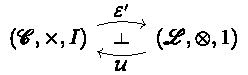
\includegraphics[width=119.0pt]{graphic-01.pdf}    
Here $\mathcal{U}$ represents the forgetful functor from linear to general maps; see Definition 8 for the full hypotheses. We consider differentiation as a functor from the coslice of the category of differentiable maps under the terminal object to the category of linear maps. The coslice category $(I\downarrow\mathscr{C})$ can be thought of as the category of pointed objects, meaning each object $A$ comes equipped with a point $a:I\>\vcenter{\hbox{
\includegraphics[height=8.3pt]{inline-07.pdf}}}\>A$ and morphisms respect these. We re-express models of $\mathrm{DiLL}$ in terms of models of $\mathrm{LL}$ equipped with a functor\par
    \[\mathcal{D}:(I\downarrow\mathscr{C})\>\vcenter{\hbox{
\includegraphics[height=8.3pt]{inline-08.pdf}}}\>\mathscr{L}\]    
with the intuition that $\mathcal{D}$ maps a function $f:(a,A)\>\vcenter{\hbox{
\includegraphics[height=8.3pt]{inline-09.pdf}}}\>(f(a),B)$ to $D_{a}(f)$, its differential at the point $a$. The only constraint we impose is that $\mathcal{D}$ leaves linear maps unchanged, (11). This simplifies both the pairwise presentation of differentiable programming (equation (2)) and the non-functorial transformation $\overline{\mathsf{d}}$ of differential categories. We will show that this definition is equivalent to that coming from differential categories up to a pointed version of the chain rule; the converse is straightforward (Proposition 27).\par
 
% END S1.p5
 
% BEGIN S1.p6
 
This approach also yields insights into how related constructions from analysis, most notably integration, can be realised in models of LL. We demonstrate this by using the slice category $(I\downarrow\mathscr{C})$ to present the fundamental theorem of analysis as an adjunction.\par
 
% END S1.p6
 
% BEGIN S1.SS0.SSS0.P0.SPx1
 
\par\medskip\noindent\textbf{Related work.}\par
 
% BEGIN S1.SS0.SSS0.P0.SPx1.p1
 
Work on differential categories [2], cartesian differential categories [3] and tangent categories [8] have been successful in categorifying differentiation from a mathematical perspective, but place models of $\mathrm{DiLL}$ as the strictest in the hierarchy of categorical definitions. Our use of coslice categories in the context of $\mathrm{DiLL}$ is novel, to our knowledge, although the dual construction of slice categories appears in various places: in reverse cartesian differential categories, partial differentials are defined on slice objects [9], and slice categories are extensively used in modeling dependent type theory. We hope our work encourages research into the relationship between differentiation and dependent types.\par
 
% END S1.SS0.SSS0.P0.SPx1.p1
 
% END S1.SS0.SSS0.P0.SPx1
 
% BEGIN S1.SS0.SSS0.P0.SPx2
 
\par\medskip\noindent\textbf{Outline and contributions.}\par
 
% BEGIN S1.SS0.SSS0.P0.SPx2.p1
 
We provide background material on differential categories in Section 2. The core results of our study are presented in Section 3, where we define $\mathcal{D}$ as a functor on the coslice $(I\downarrow\mathscr{C})$, and demonstrate that with a few assumptions, it induces the structure of a differential category on $\mathscr{L}$. We formulate categorical models of $\mathrm{DiLL}$ with a functorial definition of differentiation (Definition 15), which we prove to be equivalent to differential storage categories under some hypotheses (Proposition 26 and Proposition 27).\par
 
% END S1.SS0.SSS0.P0.SPx2.p1
 
% BEGIN S1.SS0.SSS0.P0.SPx2.p2
 
In Section 4, we first review the existing presentations of integration and fundamental theorems of analysis in differential categories, then show that the coslice construction allows for a new presentation as an adjunction between $(I\downarrow\mathscr{C})$ and $\mathscr{L}$ (Proposition 34). Finally, in Section 5, we discuss potential future work.\par
 
% END S1.SS0.SSS0.P0.SPx2.p2
 
% END S1.SS0.SSS0.P0.SPx2
 
% END S1


% BEGIN S2
 
\par\medskip\noindent\textbf{2 Preliminaries}\par
 
% BEGIN S2.p1
 
In this section, we give a quick introduction to the syntax and semantics of $\mathrm{DiLL}$. For readers familiar with $\mathrm{DiLL}$, we note that Definition 4 is the only one technically necessary to the rest of the paper; the rest of this section serves as motivation and historical introduction.\par
 
% END S2.p1
 
% BEGIN S2.p2
 
Linear Logic [15] ($\mathrm{LL}$) is the result of a decomposition of Intuitionistic Logic via an involutive linear negation. Along with multiplicative and additive versions of conjunction and disjunction, it introduces the exponential connective $\oc$ and its dual $\wn$. Some important intuition for working in $\mathrm{LL}$ coming from the Curry-Howard correspondence is that a proof of a sequent of the form $A\vdash B$ corresponds to the construction of a linear function from $A$ to $B$, while a proof of $\oc A\vdash B$ constructs a non-linear function from $A$ to $B$. When modelling $\mathrm{LL}$ in vector spaces, these intuitions are literally valid, in that a proof of $A\vdash B$ is interpreted as a linear map and a proof of $\oc A\vdash B$ is interpreted as (the transpose across the linear–non-linear adjunction of) a not-necessarily-linear map.\par
 
% END S2.p2
 
% BEGIN S2.p3
 
$\mathrm{DiLL}$ [12] adds to $\mathrm{LL}$ new rules on the connective $\oc$, expressing the fact that one is able to transform a non-linear proof into a linear one. While $\mathrm{LL}$ features a dereliction rule (${\mathsf{d}}$), $\mathrm{DiLL}$ introduces a codereliction rule ($\overline{\mathsf{d}}$) which acts like differentiation at $0$ into the logic:\par
 
\begin{center}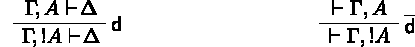
\includegraphics[width=0.95\linewidth,height=0.45\textheight,keepaspectratio]{graphic-02.pdf}\end{center}
 
% END S2.p3
 
% BEGIN S2.p4
 
This creates a duality between linear and non-linear maps in $\mathrm{DiLL}$. We recall also the exponential rules of $\mathrm{LL}$ called respectively weakening (${\mathsf{w}}$), contraction (${\mathsf{c}}$) and promotion (${\mathsf{p}}$). $\mathrm{DiLL}$ adds to these dual rules of coweakening ($\overline{\mathsf{w}}$) and cocontraction ($\overline{\mathsf{c}}$).\par
 
% END S2.p4
 
% BEGIN S2.p5
 
\begin{center}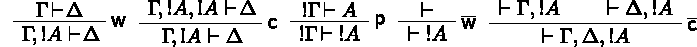
\includegraphics[width=0.95\linewidth,height=0.45\textheight,keepaspectratio]{graphic-03.pdf}\end{center}
 
% END S2.p5
 
% BEGIN S2.p6
 
Since the focus of this paper is on categorical models rather than the proof theory of these logics, we will not give a full presentation of the syntax of $\mathrm{DiLL}$; we omit the cut elimination rules and the corresponding commutative diagrams between their interpretation as these are direct translations of differential calculus rules. We refer the reader to the survey of Ehrhard [11] for a complete introduction. Let us now turn to the categorical models.\par
 
% END S2.p6
 
% BEGIN Thmtheorem1
 
\par\medskip\noindent\textbf{Definition 1.}\par
 
% BEGIN Thmtheorem1.p1
 
A Seely category [19] is a monoidal closed category $(\mathscr{L},\otimes,1)$ with finite products and a comonad $(\oc,{\mathsf{d}},\nu)$ such that $\oc$ is a (strong) monoidal functor\par
    \[\oc:(\mathscr{L},\times,\top)\>\vcenter{\hbox{
\includegraphics[height=8.3pt]{inline-10.pdf}}}\>(\mathscr{L},\otimes,1)\]    
where $\top$ denotes a terminal object. Monoidality of $\oc$ means we have “Seely isomorphisms”:\par
    \[\chi_{A,B}:\oc A\otimes\oc B\overset{\cong}{\multimap}\oc(A\times B)\hskip 10.0pt\text{ and }\hskip 10.0pt\chi_{0}:1\overset{\cong}{\multimap}\oc\top.\]    
Following the $\mathrm{LL}$ convention, we will denote linear maps by $\ell:A\multimap B$ and non-linear or smooth maps in the coKleisli category $\mathscr{L}_{\oc}$ by $f:A\>\vcenter{\hbox{
\includegraphics[height=8.3pt]{inline-11.pdf}}}\>B$ (note the difference in arrow head). To model classical $\mathrm{LL}$, one requires that $\mathrm{LL}$ be a $\ast$-autonomous category, with an involutive duality $(\_)^{\bot}\simeq\mathscr{L}(\_\,,1)$.\par
 
% END Thmtheorem1.p1
 
% END Thmtheorem1
 
% BEGIN S2.p7
 
The image of the diagonal map $\Delta_{E}:E\multimap E\times E$ and terminal map $n_{E}:E\multimap\top$ for the product in $\mathscr{L}$ under $\oc$ give each object of the form $\oc E$ a canonical coalgebra structure:\par
    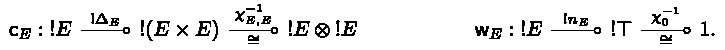
\includegraphics[width=348.0pt]{graphic-04.pdf}    
That is, Seely categories are categorical models of intuitionistic Linear Logic [17], with the above maps interpreting contraction and weakening, while dereliction is interpreted by the counit of the comonad (as suggested by the notation) and promotion is interpreted by coKleisli extension. Moreover, we recover an instance of the linear–non-linear adjunction discussed in the Introduction by constructing the coKleisli category for the comonad $\oc$.\par
 
% END S2.p7
 
% BEGIN S2.p8
 
The usual definition of categorical models of $\mathrm{DiLL}$ refines the axiomatization of Seely categories. For instance, to interpret $\overline{\mathsf{w}}$ and $\overline{\mathsf{c}}$ in this case one only needs to replace products with biproducts. This is a natural choice: to reflect the addition of rules to a logic, one adds more constructors to the categories providing the logic’s semantics.\par
 
% END S2.p8
 
% BEGIN Thmtheorem2
 
\par\medskip\noindent\textbf{Definition 2.}\par
 
% BEGIN Thmtheorem2.p1
 
A semi-additive category is a category $\mathscr{L}$ with finite products and coproducts such that the initial object is terminal and the binary product coincides with the binary coproduct. In the present paper, we denote the resulting biproduct monoidal structure by $\diamond$, with unit the zero object, denoted $0$. We also give the following names to the canonical morphisms associated to this structure:\par
    \[u_{E}:0\multimap E\qquad n_{E}:E\multimap 0\qquad\nabla_{E}:E\diamond E\multimap E\qquad\Delta_{E}:E\multimap E\diamond E\]    
% END Thmtheorem2.p1
 
% END Thmtheorem2
 
% BEGIN S2.p9
 
Note that for any object, $(E,u_{E},\nabla_{E})$ is a commutative monoid and $(E,n_{E},\Delta_{E})$ is a commutative comonoid. The hom-sets of a semi-additive category canonically carry the structure of commutative monoids: given $f,g:A\multimap B$, we may define $f+g$ to be the composite,\par
    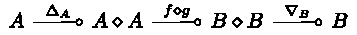
\includegraphics[width=171.0pt]{graphic-05.pdf}  (3)   
and this operation has the commutativity and associativity properties one would expect.\par
 
% END S2.p9
 
% BEGIN Thmtheorem3
 
\par\medskip\noindent\textbf{Example 3.}\par
 
% BEGIN Thmtheorem3.p1
 
The category of real vector spaces and linear maps is semi-additive, with $\diamond$ the direct sum and unit the zero vector space. The commutative monoid structure on morphisms is just the pointwise sum.\par
 
% END Thmtheorem3.p1
 
% END Thmtheorem3
 
% BEGIN S2.p10
 
There is a whole hierarchy of axiomatizations of “differential categories” [1], but we will make use of the strongest notion.\par
 
% END S2.p10
 
% BEGIN Thmtheorem4
 
\par\medskip\noindent\textbf{Definition 4.}\par
 
% BEGIN Thmtheorem4.p1
 
A differential category, called a “differential storage category” in [2] is a semi-additive Seely category $(\mathscr{L},\otimes,1)$ (with biproducts denoted as in Definition 2) in which the comonad $(\oc,{\mathsf{d}},\nu)$ is equipped with a natural transformation $\overline{\mathsf{d}}:\operatorname{id}\Rightarrow\oc$ satisfying:\par
  
\par\noindent  $\blacksquare$ 
% BEGIN S2.I1.i1.p1
 
invariance of linear maps under differentiation,\par
    \[\overline{\mathsf{d}};{\mathsf{d}}=\operatorname{id}\]  (4)   
% END S2.I1.i1.p1
 
 
\par\noindent  $\blacksquare$ 
% BEGIN S2.I1.i2.p1
 
and the generalized chain rule, requiring the following diagram to commute:\par
    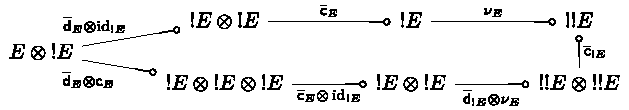
\includegraphics[width=302.0pt]{graphic-06.pdf}  (5)   
% END S2.I1.i2.p1
 
  
where $\overline{\mathsf{c}}$ and $\overline{\mathsf{w}}$ are constructed from the algebra structure on each object as follows:\par
    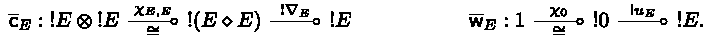
\includegraphics[width=343.0pt]{graphic-07.pdf}    
These endow $\oc E$ with coalgebra structure dualizing the algebra structure constructed earlier.222The definition given in [2] includes more equations; this presentation is equivalent by [1, Corollary 6.3].\par
 
% END Thmtheorem4.p1
 
% END Thmtheorem4
 
% BEGIN S2.p11
 
The generalized chain rule (5) captures the usual formula for composed functions,\par
    \[D_{a}(f;g)=D_{a}(f);D_{f(a)}(g).\]    
For the reader unfamiliar with differential categories, we now get a bit more into the categorical transposition of chain rule. We start with the simpler case of differentiation at $0$, the chain rule without a context, called the “alternative chain rule” $[dC.4^{\prime}]$ in [1]:\par
    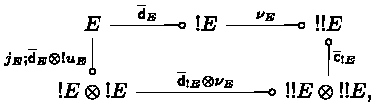
\includegraphics[width=183.0pt]{graphic-08.pdf}  (6)   
where $j_{E}:=E\multimap E\otimes 1$ is the inverse of the right unit map. The relationship becomes more apparent if we post-compose this diagram with $\oc f;g$, for $f:\oc E\multimap F$ and $g:\oc F\multimap G$. The comultiplication $\nu_{E}:\oc E\multimap\oc\oc E$ expresses composition of transposed non-linear maps: if $f$ and $g$ are respectively the transposes of non-linear maps $f^{\#},g^{\#}\in\mathscr{C}$, then $\nu_{F};\oc{f};g:\oc E\multimap G$ transpose to $f^{\#};g^{\#}$. As such, $\overline{\mathsf{d}}_{E};\nu_{E};\oc{f};g:E\multimap G$ represents the differential $D_{0}((f;g)^{\#})$. Meanwhile, by naturality of $\overline{\mathsf{c}}$ and $\overline{\mathsf{d}}$, the alternative composite can be rearranged to $\overline{\mathsf{d}}_{E};f;\overline{\mathsf{d}}_{F};j_{E};(\oc u_{E};\nu_{E};\oc f)\otimes\operatorname{id}_{F};\overline{\mathsf{c}};g$; the first two terms yield $D_{0}(f^{\#})$, while the rest translates to $D_{0}(g^{\#}(f^{\#}(0)+-))$, which by a change of variables is equal to $D_{f^{\#}(0)}(g^{\#})$. The generalized chain rule (5) adds to this set-up a parameter along which functions are not differentiated, so captures the chain rule for partial differentiation.\par
 
% END S2.p11
 
% BEGIN Thmtheorem5
 
\par\medskip\noindent\textbf{Proposition 5 ([1, Lemma 6.5]).}\par
 
% BEGIN Thmtheorem5.p1
 
The generalized chain rule 5 can be recovered from the alternative chain rule 6 if one asks for the following strength condition on $\oc$, where $m:\oc E\otimes\oc F\>\vcenter{\hbox{
\includegraphics[height=8.3pt]{inline-12.pdf}}}\>\oc(E\times F)$ represents the monoidality of $\oc$ within $(\mathscr{L},\otimes,1)$ and can be reconstructed from the Seely isomorphisms $\chi_{E,F}$.\par
    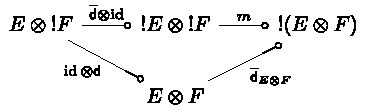
\includegraphics[width=176.0pt]{graphic-09.pdf}  (7)   
In terms of the Seely isomorphisms, this becomes a more complex condition:\par
    \[\operatorname{id}_{\oc E}\otimes\overline{\mathsf{d}}_{E};\chi_{E,E}^{-1};\overline{\mathsf{d}}_{\oc(E\diamond E)};\oc\chi;\oc(d_{E}\otimes d_{E})=\operatorname{id}_{\oc E}\otimes\overline{\mathsf{d}}_{E};\chi^{-1};\nu_{E\diamond E};\oc\chi_{E,E};\oc(d_{E}\otimes d_{E})\]    
% END Thmtheorem5.p1
 
% END Thmtheorem5
 
% BEGIN S2.p12
 
The transformations $\overline{\mathsf{c}}$, $\overline{\mathsf{w}}$ and $\overline{\mathsf{d}}$ complement the components of $\mathrm{LL}$ interpreted in a general Seely category to produce an interpretation of $\mathrm{DiLL}$. In fact, the differential categories axiomatized above are denotational models of intuitionistic $\mathrm{DiLL}$, and of classical $\mathrm{DiLL}$ when we impose the extra condition of $\ast$-autonomy on $\mathscr{L}$. The exploration of less strict axiomatizations has been fruitful in incorporating various mathematical examples from functional analysis and differential geometry into this logical framework. However, the definition above crucially does not reflect the symmetry of exponential rules in $\mathrm{DiLL}$, and does not express differentiation using the traditional objects of computer science. Notably, the chain rule is at first sight quite intricate. In this paper, we attempt to simplify this by showing that it is a consequence of functoriality in a new presentation.\par
 
% END S2.p12
 
% BEGIN S2.p13
 
Rather than merely introducing new operations such as $\overline{\mathsf{d}}$, our approach requires us to introduce new categories on top of the $\mathrm{LL}$ setup, expanding Definition 1 to an adjunction involving the coKleisli category of $\oc$ mentioned above. Nonetheless, the extension of $\mathrm{LL}$ to $\mathrm{DiLL}$ described in Definition 4 can be recovered from our construction.\par
 
% END S2.p13
 
% BEGIN S2.SS0.SSS0.P0.SPx1
 
\par\medskip\noindent\textbf{Notation.}\par
 
% BEGIN S2.SS0.SSS0.P0.SPx1.p1
 
Given a differentiable function $f:A\>\vcenter{\hbox{
\includegraphics[height=8.3pt]{inline-13.pdf}}}\>B$ between two vector spaces, we denote by $D_{a}f:A\multimap B$ the linear map corresponding to the differential of $f$ at a point $a\in A$.\par
 
% END S2.SS0.SSS0.P0.SPx1.p1
 
% BEGIN Thmtheorem6
 
\par\medskip\noindent\textbf{Example 6 (The distribution model).}\par
 
% BEGIN Thmtheorem6.p1
 
The category of convenient spaces [4] provides an illustrative example of a differential category. Formulas are interpreted by real topological vector spaces endowed with a bornology, which is a well-behaving collection of bounded sets; we shall not attempt to give detailed definitions of these structures here. The exponential $\oc A$ is interpreted as the completion of the vector space generated by the Dirac distributions,\par
    \[\llbracket{\oc A}\rrbracket:=\overline{\langle\delta_{x}\rangle_{x\in\llbracket{A}\rrbracket}}.\]    
The Dirac distribution $\delta_{x}$, defined by $f\in\mathscr{C}(E,\mathbb{R})\mapsto f(x)$, is formally an object of the dual $\mathscr{C}(E,\mathbb{R})^{\prime}$ of the space of smooth functions, otherwise known as the space of distributions of compact support over $E$ [18]. As the Dirac distributions form a linearly independent family of distributions, to define linear morphisms on $\oc E$ it is enough to specify their value on Diracs and then extend linearly and continuously to the completion. As such, the components of $\mathrm{DiLL}$ are interpreted as follows:\par
 
\begin{center}\resizebox{\linewidth}{!}{$\begin{aligned}\displaystyle{\mathsf{d}} & \displaystyle:\delta_{x}\in\oc E\mapsto x\in E & \displaystyle{\mathsf{c}} & \displaystyle:\delta_{x}\in\oc E\mapsto\delta_{x}\otimes\delta_{x}\in\oc E\otimes\oc E & \displaystyle{\mathsf{w}} & \displaystyle:\delta_{x}\in\oc E\mapsto 1\in\mathbb{R}\\\displaystyle\overline{\mathsf{d}} & \displaystyle:x\in E\mapsto D_{0}(\_)(x)\in\oc E & \displaystyle\overline{\mathsf{c}} & \displaystyle:\delta_{x}\otimes\delta_{y}\in\oc E\otimes\oc E\mapsto\delta_{x+y}\in\oc E & \displaystyle\overline{\mathsf{w}} & \displaystyle:1\in\mathbb{R}\mapsto\delta_{0}\in\oc E\\\displaystyle\nu & \displaystyle:\delta_{x}\in\oc E\mapsto\delta_{\delta_{x}}\in\oc\oc E\end{aligned}$}\end{center}
 
Convenient spaces do not form a $\ast$-autonomous category, and constructing $\ast$-autonomous smooth models of $\mathrm{DiLL}$ with a non-trivial duality is tricky, often requiring compromise on the interpretation of the other components of $\mathrm{DiLL}$, such as [10] which features an ad-hoc construction to allow differentiation. An alternative work-around for this issue is to construct polarized models of $\mathrm{DiLL}$ [16].\par
 
% END Thmtheorem6.p1
 
% END Thmtheorem6
 
% BEGIN Thmtheorem7
 
\par\medskip\noindent\textbf{Example 7.}\par
 
% BEGIN Thmtheorem7.p1
 
We denote by $\mathsf{REL}$ the category of sets and relations. The interpretation of $\mathrm{LL}$ in $\mathsf{REL}$ produces the well-known, historical “relational model”. The tensor product is given by the cartesian product of sets, $X\otimes Y=X\times Y$ and the product (which coincides with the coproduct) is given by the disjoint union of sets $X\sqcup Y$. The exponential $\oc$ is interpreted by finite multisets: $\oc X=\mathcal{M}_{f}(X)$, the set of all finite multisets of $X$. The dereliction ${\mathsf{d}}_{X}\subseteq\oc X\times X$ and codereliction $\overline{\mathsf{d}}_{X}\subseteq X\times\oc X$ respectively put in relation elements with singleton multisets containing them, and reciprocally. The contraction ${\mathsf{c}}_{X}\subseteq\oc X\times(\oc X\times\oc X)$ and cocontraction $\overline{\mathsf{c}}_{X}\subseteq(\oc X\times\oc X)\times\oc X$ relate pairs of finite multisets to their disjoint union, while the weakening $\mathsf{w}_{X}\subseteq\oc X\times\{\ast\}$ and coweakening $\overline{\mathsf{w}}_{X}\subseteq\{\ast\}\times\oc X$ relate $\ast$ to the empty multiset. The co-multiplication of the co-monad $\oc$ is $\nu_{X}\subseteq\oc X\times\oc\oc X$, relates a finite multiset to each finite multiset of finite multisets of which it is the disjoint union.\par
 
% END Thmtheorem7.p1
 
% END Thmtheorem7
 
% END S2.SS0.SSS0.P0.SPx1
 
% END S2


% BEGIN S3
 
\par\medskip\noindent\textbf{3 Differentiation on the coslice}\par
 
% BEGIN S3.p1
 
This section represents the heart of this paper: here we will start from a linear–non-linear adjunction and show how defining a functor from a coslice of the non-linear category $\mathscr{C}$ to the linear category $\mathscr{L}$ makes $\mathscr{L}$ into a differential category, up to a well-pointed assumption.\par
 
% END S3.p1
 
% BEGIN Thmtheorem8
 
\par\medskip\noindent\textbf{Definition 8.}\par
 
% BEGIN Thmtheorem8.p1
 
For the purposes of the present paper, a linear–non-linear adjunction is an adjunction:\par
    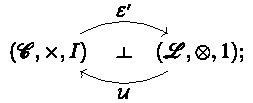
\includegraphics[width=122.0pt]{graphic-10.pdf}  (8)   
in which:\par
  
\par\noindent  $\blacksquare$ 
% BEGIN S3.I1.i1.p1
 
$\mathscr{L}$ is both monoidal closed and semi-additive;\par
 
% END S3.I1.i1.p1
 
 
\par\noindent  $\blacksquare$ 
% BEGIN S3.I1.i2.p1
 
$\mathscr{C}$ has cartesian monoidal structure;\par
 
% END S3.I1.i2.p1
 
 
\par\noindent  $\blacksquare$ 
% BEGIN S3.I1.i3.p1
 
$\mathcal{E}^{\prime}$ is a strong monoidal functor, so $\mathcal{E}^{\prime}(A\times B)\cong\mathcal{E}^{\prime}(A)\otimes\mathcal{E}^{\prime}(B)$ and $1\cong\mathcal{E}^{\prime}(I)$.\par
 
% END S3.I1.i3.p1
 
  
This adds hypothesis to the usual notion of linear-non-linear adjunction, in which the semi-additivity is not required and the adjunction is only lax monoidal [17, Definition 21].\par
 
% END Thmtheorem8.p1
 
% END Thmtheorem8
 
% BEGIN S3.SS0.SSS0.P0.SPx1
 
\par\medskip\noindent\textbf{Notation.}\par
 
% BEGIN S3.SS0.SSS0.P0.SPx1.p1
 
We denote the endofunctor on $\mathscr{L}$ from the adjunction 8 by $\oc:=\mathcal{E}^{\prime}\circ\mathcal{U}$, the unit by $\eta:\operatorname{id}_{\mathscr{C}}\Rightarrow\mathcal{U}\circ\mathcal{E}^{\prime}$ and the counit by ${\mathsf{d}}:\oc\Rightarrow\operatorname{id}_{\mathscr{L}}$. We moreover write $\nu=\mathcal{E}^{\prime}\eta_{\mathcal{U}}$ for the comultiplication of the induced comonad $(\oc,{\mathsf{d}},\nu)$ on $\mathscr{L}$. We denote $f\in\mathscr{C}(A,B)$ by $f:A\>\vcenter{\hbox{
\includegraphics[height=8.3pt]{inline-14.pdf}}}\>B$ and $\ell\in\mathscr{L}(E,F)$ by $\ell:E\multimap F$, which is consistent with our notation for Seely categories in the special case where $\mathscr{C}$ is the coKleisli category of $\oc$. Note that $\mathcal{U}$ preserves products, being a right adjoint. For notational convenience, we work as if $\mathcal{U}$ and $\mathcal{E}^{\prime}$ are strictly monoidal, in the sense that we suppress the isomorphisms $\mathcal{U}(A\diamond B)\cong\mathcal{U}(A)\times\mathcal{U}(B)$ and $\mathcal{E}^{\prime}(A\times B)\cong\mathcal{E}^{\prime}(A)\otimes\mathcal{E}^{\prime}(B)$. With this convention, the projection map $\pi_{1}:A\diamond B\multimap A$ satisfies $\mathcal{U}(\pi_{1})=\pi_{1}:\mathcal{U}(A)\times\mathcal{U}(B)\>\vcenter{\hbox{
\includegraphics[height=8.3pt]{inline-15.pdf}}}\>\mathcal{U}(A)$ and moreover (considering the case $B=0$) $\mathcal{U}$ preserves the left and right unit maps for $0$ on the nose.\par
 
% END S3.SS0.SSS0.P0.SPx1.p1
 
% BEGIN Thmtheorem9
 
\par\medskip\noindent\textbf{$\blacktriangleright$ Remark 9.}\par
 
% BEGIN Thmtheorem9.p1
 
We will not actually use the fact that the monoidal structure $\otimes$ on $\mathscr{L}$ is closed, but we wished to ensure the hypotheses in the various definitions lined up.\par
 
% END Thmtheorem9.p1
 
% END Thmtheorem9
 
% BEGIN Thmtheorem10
 
\par\medskip\noindent\textbf{Example 10.}\par
 
% BEGIN Thmtheorem10.p1
 
The distribution model of Example 3 can also be understood from the adjunction point of view instead of the comonadic point of view. Let $\mathscr{C}$ be the category whose objects are convenient vector spaces and whose morphisms are smooth functions and $\mathscr{L}$ the category of convenient vector spaces and linear maps. In adjunction (8), $\mathcal{E}^{\prime}$ is interpreted via $\mathcal{E}^{\prime}(E):=\overline{\langle\delta_{x}\rangle_{x\in\llbracket{E}\rrbracket}}$, that is the space generated by Dirac distributions on $E$, and $\mathcal{U}$ is the forgetful functor. $\mathscr{C}$ is a cartesian closed category, $\mathscr{L}$ is monoidal closed and $(\mathcal{E}^{\prime}\dashv U)$ is a strong monoidal adjunction.\par
 
% END Thmtheorem10.p1
 
% END Thmtheorem10
 
% BEGIN Thmtheorem11
 
\par\medskip\noindent\textbf{Lemma 11 ([17]).}\par
 
% BEGIN Thmtheorem11.p1
 
Given a linear–non-linear adjunction as in Definition 8, $\mathscr{L}$ acquires the structure of a Seely category.\par
 
% END Thmtheorem11.p1
 
% END Thmtheorem11
 
% BEGIN S3.SS0.SSS0.P0.SPx1.p2
 
As such, we can interpret the ingredients of Differential Linear Logic, ${\mathsf{c}},{\mathsf{w}},\overline{\mathsf{c}},\overline{\mathsf{w}}$ and ${\mathsf{d}}$, as we did in Section 2. In order to interpret differentiation, we need to expose further structure. To begin with, we observe that the semi-additive structure on $\mathscr{L}$ is partially preserved by $\mathcal{U}$.\par
 
% END S3.SS0.SSS0.P0.SPx1.p2
 
% BEGIN Thmtheorem12
 
\par\medskip\noindent\textbf{Proposition 12.}\par
 
% BEGIN Thmtheorem12.p1
 
Suppose that we are given a linear–non-linear adjunction as in Definition 8. For objects $E\in\mathscr{L}$ and $A\in\mathscr{C}$, $\mathscr{C}(A,\mathcal{U}(E))$ has a distinguished element,\par
    \[0_{A,E}:A\xrightarrow{n_{A}}I\xrightarrow{\mathcal{U}(u_{E})}\mathcal{U}(E),\]    
where $n_{A}$ is the unique morphism. This is the identity element of a commutative monoid structure on $\mathscr{C}(A,\mathcal{U}(E))$.\par
 
% END Thmtheorem12.p1
 
% END Thmtheorem12
 
% END S3.SS0.SSS0.P0.SPx1
 
% BEGIN S3.SS0.SSS0.P0.SPx2
 
\par\medskip\noindent\textbf{Proof.}\par
 
% BEGIN S3.SS0.SSS0.P0.SPx2.p1
 
For $f,g:A\rightrightarrows\mathcal{U}(E)$, we define their sum using the codiagonal map:\par
    \[f\boxplus g:A\xrightarrow{\langle f,g\rangle}\mathcal{U}(E\diamond E)\xrightarrow{\mathcal{U}(\nabla_{E})}\mathcal{U}(E).\]  (9)   
To show that $0_{A,E}$ is the identity element, consider the transpose of $f\boxplus 0_{A,E}$:\par
    \[\mathcal{E}^{\prime}(\langle f,0_{A,E})\rangle);\mathcal{E}^{\prime}(\mathcal{U}(\nabla_{E}));{\mathsf{d}}_{E}=\mathcal{E}^{\prime}(f)\otimes\overline{\mathsf{w}}_{E};\overline{\mathsf{c}}_{E};{\mathsf{d}}_{E}\]    
by monoidality of $\mathcal{E}^{\prime}$. The bialgebra laws over $\oc E$, as described for example in [1, Section 7] give us $\operatorname{id}_{E}\otimes\overline{\mathsf{w}}_{E};\overline{\mathsf{c}}_{E}=\operatorname{id}_{E}$ and as such $\mathcal{E}^{\prime}(f)\otimes\overline{\mathsf{w}}_{E};\overline{\mathsf{c}}_{E};{\mathsf{d}}_{E}=\mathcal{E}^{\prime}(f);{\mathsf{d}}_{E}$, the transpose of $f$, so $f=f\boxplus 0_{A,E})$ as required. $\hfill\blacktriangleleft$\par
 
% END S3.SS0.SSS0.P0.SPx2.p1
 
% BEGIN S3.SS0.SSS0.P0.SPx2.p2
 
Next we formalize the category of pointed objects of $\mathscr{C}$.\par
 
% END S3.SS0.SSS0.P0.SPx2.p2
 
% BEGIN Thmtheorem13
 
\par\medskip\noindent\textbf{Definition 13.}\par
 
% BEGIN Thmtheorem13.p1
 
Suppose that $\mathscr{L}$ is a category with a zero object $0$, that $\mathscr{C}$ is a category with terminal object $I$ and that we are given a functor $\mathcal{U}:\mathscr{L}\>\vcenter{\hbox{
\includegraphics[height=8.3pt]{inline-16.pdf}}}\>\mathscr{C}$ sending $0$ to $I$.\par
 
% END Thmtheorem13.p1
 
% BEGIN Thmtheorem13.p2
 
Recall that the coslice category $(I\downarrow\mathscr{C})$ is defined as follows. The objects of $(I\downarrow\mathscr{C})$ are pairs $(A,a)$ with $A\in\mathscr{C}$ and $a\in\mathscr{C}(I,A)$, and morphisms $(A,a)\>\vcenter{\hbox{
\includegraphics[height=8.3pt]{inline-17.pdf}}}\>(B,b)$ are morphisms $g:A\>\vcenter{\hbox{
\includegraphics[height=8.3pt]{inline-18.pdf}}}\>B$ such that $a;g=b$.\par
 
% END Thmtheorem13.p2
 
% BEGIN Thmtheorem13.p3
 
We may similarly construct the coslice category $(I\downarrow\mathcal{U})$ where objects are instead pairs $(E,a)$ with $E\in\mathscr{L}$ and $a\in\mathscr{C}(I,\mathcal{U}(E))$, and morphisms $(E,a)\>\vcenter{\hbox{
\includegraphics[height=8.3pt]{inline-19.pdf}}}\>(F,b)$ consist of $\ell\in\mathscr{L}(E,F)$ with $a;\mathcal{U}(\ell)=b$.\par
 
% END Thmtheorem13.p3
 
% END Thmtheorem13
 
% END S3.SS0.SSS0.P0.SPx2
 
% BEGIN S3.SS0.SSS0.P0.SPx3
 
\par\medskip\noindent\textbf{Notation.}\par
 
% BEGIN S3.SS0.SSS0.P0.SPx3.p1
 
In order to more explicitly keep track of the points involved in a morphism of $(I\downarrow\mathscr{C})$, we denote a morphism $g:(A,a)\>\vcenter{\hbox{
\includegraphics[height=8.3pt]{inline-20.pdf}}}\>(B,b)$ by $\left(a\rceil g\right)$.\par
 
% END S3.SS0.SSS0.P0.SPx3.p1
 
% BEGIN S3.SS0.SSS0.P0.SPx3.p2
 
The coslice categories $(I\downarrow\mathscr{C})$ and $(I\downarrow\mathcal{U})$ come equipped with projection functors to $\mathscr{C}$ and $\mathscr{L}$ which respectively forget the points; we denote both by $\Pi$. Moreover, $\mathcal{U}$ induces a functor $(I\downarrow\mathcal{U})\>\vcenter{\hbox{
\includegraphics[height=8.3pt]{inline-21.pdf}}}\>(I\downarrow\mathscr{C})$ which we denote by $\downarrow\mathcal{U}$, mapping $(E,a)$ to $(\mathcal{U}(E),a)$. Putting these together, we get:\par
    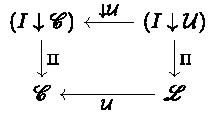
\includegraphics[width=103.0pt]{graphic-11.pdf}  (10)   
% END S3.SS0.SSS0.P0.SPx3.p2
 
% BEGIN Thmtheorem14
 
\par\medskip\noindent\textbf{Example 14.}\par
 
% BEGIN Thmtheorem14.p1
 
Let’s see how differentiation can be interpreted in Example 10 using the coslice construction. In this case $I$ is the zero vector space $\{0\}$ and $(I\downarrow\mathscr{C})$ is the category of pairs $(A,a)$, where $a$ is a vector in $A$. Differentiation defines a functor $\mathcal{D}:(I\downarrow\mathscr{C})\>\vcenter{\hbox{
\includegraphics[height=8.3pt]{inline-22.pdf}}}\>\mathscr{L}$ as follows: an object $a:I\>\vcenter{\hbox{
\includegraphics[height=8.3pt]{inline-23.pdf}}}\>A$ is mapped to $A$ and an arrow $\left(a\rceil g\right)$ is sent to the linear map $D_{a}f:A\multimap B$. The chain rule exactly translates to functoriality of $\mathcal{D}$. Indeed, morphisms $\left(a\rceil g\right)$ and $\left(b\rceil h\right)$ compose if and only if $b=g(a)$ and then we have\par
    \[\mathcal{D}\left(a\rceil g;h\right)=D_{a}(g;h)=D_{a}g;D_{g(a)}h=\mathcal{D}\left(a\rceil g\right);\mathcal{D}\left(g(a)\rceil h\right).\]    
% END Thmtheorem14.p1
 
% END Thmtheorem14
 
% BEGIN S3.SS0.SSS0.P0.SPx3.p3
 
Example 14 contains the essential idea of the present section. As we shall shortly see, there will be no need to independently construct a codereliction operator once we equip our adjunction with a differentiation functor, since codereliction can be recovered from $\mathcal{D}$ as differentiation at $0$.\par
 
% END S3.SS0.SSS0.P0.SPx3.p3
 
% BEGIN Thmtheorem15
 
\par\medskip\noindent\textbf{Definition 15.}\par
 
% BEGIN Thmtheorem15.p1
 
A functorial model of differentiation consists a linear–non-linear adjunction $(\mathcal{E}^{\prime}\dashv\mathcal{U})$ between $\mathscr{L}$ and $\mathscr{C}$ equipped with a functor $\mathcal{D}:(I\downarrow\mathscr{C})\>\vcenter{\hbox{
\includegraphics[height=8.3pt]{inline-24.pdf}}}\>\mathscr{L}$ such that\par
    \[\mathcal{D}\circ{\downarrow\!\mathcal{U}}=\Pi,\]  (11)   
which is to say that the following triangle (ignoring the dashed functors) commutes:\par
    
\begin{center}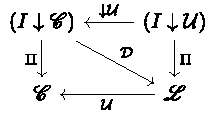
\includegraphics[width=0.95\linewidth,height=0.45\textheight,keepaspectratio]{graphic-12.pdf}\end{center}
    
% END Thmtheorem15.p1
 
% END Thmtheorem15
 
% BEGIN Thmtheorem16
 
\par\medskip\noindent\textbf{$\blacktriangleright$ Remark 16.}\par
 
% BEGIN Thmtheorem16.p1
 
The choice of name in Definition 15 is not intended to seem grandiose: as we shall see, these categories do not quite constitute models of $\mathrm{DiLL}$ in general. As discussed in the introduction, the idea that the chain rule is compositional on pairs of objects is well-established [13]. Here we explore another presentation of differentiation as a functor compatible with linear–non-linear adjunctions as models of Linear Logic.\par
 
% END Thmtheorem16.p1
 
% END Thmtheorem16
 
% BEGIN S3.SS0.SSS0.P0.SPx3.p4
 
More explicitly, (11) says that for any object $E$ of $\mathscr{L}$ and point $a:I\>\vcenter{\hbox{
\includegraphics[height=8.3pt]{inline-25.pdf}}}\>\mathcal{U}(E)$ we have $\mathcal{D}\left(a\rceil\mathcal{U}(E)\right)=E$, and that for any arrow $\ell:E\multimap F$ in $\mathscr{L}$ we have $\mathcal{D}\left(a\rceil\mathcal{U}(\ell)\right)=\ell$. This identity also implies that $\mathcal{D}$ preserves products of objects in $\mathcal{U}(\mathscr{L})$, in the following sense:\par
 
% END S3.SS0.SSS0.P0.SPx3.p4
 
% BEGIN Thmtheorem17
 
\par\medskip\noindent\textbf{Lemma 17.}\par
 
% BEGIN Thmtheorem17.p1
 
The functor $\mathcal{D}$ in Definition 15 preserves limits of objects in the image of ${\downarrow\!\mathcal{U}}$. In particular, for $h_{1}:A\>\vcenter{\hbox{
\includegraphics[height=8.3pt]{inline-26.pdf}}}\>\mathcal{U}(E_{1})$ and $h_{2}:A\>\vcenter{\hbox{
\includegraphics[height=8.3pt]{inline-27.pdf}}}\>\mathcal{U}(E_{2})$ in $\mathscr{C}$ and $a:I\>\vcenter{\hbox{
\includegraphics[height=8.3pt]{inline-28.pdf}}}\>A$, we have:\par
    \[\mathcal{D}\left(a\rceil\langle h_{1},h_{2}\rangle\right)=\langle\mathcal{D}\left(a\rceil h_{1}\right),\mathcal{D}\left(a\rceil h_{2}\right)\rangle.\]  (12)   
% END Thmtheorem17.p1
 
% END Thmtheorem17
 
% END S3.SS0.SSS0.P0.SPx3
 
% BEGIN S3.SS0.SSS0.P0.SPx4
 
\par\medskip\noindent\textbf{Proof.}\par
 
% BEGIN S3.SS0.SSS0.P0.SPx4.p1
 
A short proof is that $\Pi$ creates limits and ${\downarrow\!\mathcal{U}}$ preserves them (because $\mathcal{U}$ does), whence the identity (11) forces $\mathcal{D}$ to preserve them. $\hfill\blacktriangleleft$\par
 
% END S3.SS0.SSS0.P0.SPx4.p1
 
% BEGIN Thmtheorem18
 
\par\medskip\noindent\textbf{Proposition 18.}\par
 
% BEGIN Thmtheorem18.p1
 
Given morphisms in $\mathscr{C}$, $I\xrightarrow{a}A_{1}\xrightarrow{g_{1}}A_{2}\xrightarrow{g_{2}}A_{3},$ we have:\par
 
\begin{center}\resizebox{\linewidth}{!}{$\begin{aligned}\displaystyle\mathcal{D}\left(a\rceil g_{1};g_{2}\right) & \displaystyle=\mathcal{D}\left(a\rceil g_{1}\right);\mathcal{D}\left(a;g_{1}\rceil g_{2}\right).\end{aligned}$}\end{center}
 
Similarly, given:\par
    
\begin{center}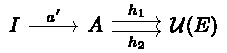
\includegraphics[width=0.95\linewidth,height=0.45\textheight,keepaspectratio]{graphic-13.pdf}\end{center}
    
we have,\par
    \[\mathcal{D}\left(a^{\prime}\rceil h_{1}\boxplus h_{2}\right)=\mathcal{D}\left(a^{\prime}\rceil h_{1}\right)+\mathcal{D}\left(a^{\prime}\rceil h_{2}\right).\]  (14)   
% END Thmtheorem18.p1
 
% END Thmtheorem18
 
% END S3.SS0.SSS0.P0.SPx4
 
% BEGIN S3.SS0.SSS0.P0.SPx5
 
\par\medskip\noindent\textbf{Proof.}\par
 
% BEGIN S3.SS0.SSS0.P0.SPx5.p1
 
The first identity is an immediate consequence of functoriality of $\mathcal{D}$. For the second, the definition of $h_{1}\boxplus h_{2}$ produces the following diagram:\par
    
\begin{center}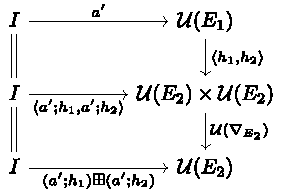
\includegraphics[width=0.95\linewidth,height=0.45\textheight,keepaspectratio]{graphic-14.pdf}\end{center}
    
Applying $\mathcal{D}$, the upper square is mapped to $\langle\mathcal{D}\left(a^{\prime}\rceil h_{1}\right),\mathcal{D}\left(a^{\prime}\rceil h_{2}\right)\rangle$ by Lemma 17 and the lower square is mapped to $\nabla_{E_{2}}$ by (11), yielding the desired sum, as required. $\hfill\blacktriangleleft$ As such, $\mathcal{D}$ satisfies the chain rule and is linear with respect to the additive structure on morphisms. It follows that $\mathcal{D}$ interacts well with products of morphisms too:\par
 
% END S3.SS0.SSS0.P0.SPx5.p1
 
% BEGIN Thmtheorem19
 
\par\medskip\noindent\textbf{Corollary 19.}\par
 
% BEGIN Thmtheorem19.p1
 
Let $g_{1}:\mathcal{U}(E^{\prime}_{1})\>\vcenter{\hbox{
\includegraphics[height=8.3pt]{inline-29.pdf}}}\>\mathcal{U}(E)$ and $g_{2}:\mathcal{U}(E^{\prime}_{2})\>\vcenter{\hbox{
\includegraphics[height=8.3pt]{inline-30.pdf}}}\>\mathcal{U}(E)$ and $a=\langle a_{1},a_{2}\rangle:I\>\vcenter{\hbox{
\includegraphics[height=8.3pt]{inline-31.pdf}}}\>\mathcal{U}(E^{\prime}_{1})\times\mathcal{U}(E^{\prime}_{2})$. Then we have:\par
    \[\mathcal{D}\left(a\rceil g_{1}\times g_{2}\right)=\mathcal{D}\left(a_{1}\rceil
g_{1}\right)\diamond\mathcal{D}\left(a_{2}\rceil h_{2}\right).\]  (15)   
% END Thmtheorem19.p1
 
% END Thmtheorem19
 
% END S3.SS0.SSS0.P0.SPx5
 
% BEGIN S3.SS0.SSS0.P0.SPx6
 
\par\medskip\noindent\textbf{Proof.}\par
 
% BEGIN S3.SS0.SSS0.P0.SPx6.p1
 
By definition, $g_{1}\times g_{2}=\langle\mathcal{U}(\pi_{1});g_{1},\mathcal{U}(\pi_{2});g_{2}\rangle$. Thus by Lemma 17,\par
    \[\mathcal{D}\left(a\rceil g_{1}\times g_{2}\right)=\langle\mathcal{D}\left(a\rceil\mathcal{U}(\pi_{1});g_{1}\right),\mathcal{D}\left(a\rceil\mathcal{U}(\pi_{2});g_{2}\right)\rangle.\]    
We have: $\mathcal{D}\left(a\rceil\mathcal{U}(\pi_{1});g_{1}\right)=\mathcal{D}\left(a\rceil\mathcal{U}(\pi_{1})\right);\mathcal{D}\left(a;\mathcal{U}(\pi_{1})\rceil g_{1}\right)=\pi_{1};\mathcal{D}\left(a_{1}\rceil g_{1}\right),$ by (11) and similarly for $\mathcal{D}\left(a\rceil\mathcal{U}(\pi_{2});g_{2}\right)$, whence we recover the claimed product of morphisms. $\hfill\blacktriangleleft$\par
 
% END S3.SS0.SSS0.P0.SPx6.p1
 
% BEGIN S3.SS0.SSS0.P0.SPx6.p2
 
Comparing with differential categories, the only thing missing from $\mathscr{L}$ to make it a differential category is a codereliction $\overline{\mathsf{d}}:\operatorname{id}\Rightarrow\oc$ satisfying the required identities.\par
 
% END S3.SS0.SSS0.P0.SPx6.p2
 
% BEGIN Thmtheorem20
 
\par\medskip\noindent\textbf{Definition 20.}\par
 
% BEGIN Thmtheorem20.p1
 
For $E$ an object of $\mathscr{L}$, we define: $\overline{\mathsf{d}}_{E}:=\mathcal{D}\left(\mathcal{U}(u_{E})\rceil\eta_{\mathcal{U}(E)}\right):E\multimap\oc E.$\par
 
% END Thmtheorem20.p1
 
% END Thmtheorem20
 
% BEGIN Thmtheorem21
 
\par\medskip\noindent\textbf{Lemma 21.}\par
 
% BEGIN Thmtheorem21.p1
 
The transformation $\overline{\mathsf{d}}:\operatorname{id}_{\mathscr{L}}\Rightarrow\oc$ is natural.\par
 
% END Thmtheorem21.p1
 
% END Thmtheorem21
 
% END S3.SS0.SSS0.P0.SPx6
 
% BEGIN S3.SS0.SSS0.P0.SPx7
 
\par\medskip\noindent\textbf{Proof.}\par
 
% BEGIN S3.SS0.SSS0.P0.SPx7.p1
 
We have a functor $R:\mathscr{L}\>\vcenter{\hbox{
\includegraphics[height=8.3pt]{inline-32.pdf}}}\>(I\downarrow\mathscr{C})$ sending $E$ to $\mathcal{U}(u_{E}):I\>\vcenter{\hbox{
\includegraphics[height=8.3pt]{inline-33.pdf}}}\>\mathcal{U}(E)$ and $\ell:E\multimap F$ to $\left(\mathcal{U}(u_{E})\rceil\mathcal{U}(\ell)\right)$; this is a section of $\mathcal{D}$. By inspection, $\eta_{\mathcal{U}(-)}$ lifts to a natural transformation $R\Rightarrow R\circ\oc$, and $\overline{\mathsf{d}}$ is the result of applying $\mathcal{D}$ to this lifting, so is natural as required. $\hfill\blacktriangleleft$\par
 
% END S3.SS0.SSS0.P0.SPx7.p1
 
% BEGIN S3.SS0.SSS0.P0.SPx7.p2
 
We denote by $\ell^{\#}:\mathcal{U}(E)\>\vcenter{\hbox{
\includegraphics[height=8.3pt]{inline-34.pdf}}}\>\mathcal{U}(F)$ the transpose of a morphism $\ell:\oc E\multimap F$ in $\mathscr{L}$ across the adjunction $(\mathcal{E}^{\prime}\dashv\mathcal{U})$. Since $\ell^{\#}=\eta_{U(E)};\mathcal{U}(\ell)$, using Proposition 18, the definition of $\overline{\mathsf{d}}_{E}$ and (11) we have:\par
    \[\mathcal{D}\left(\mathcal{U}(u_{E})\rceil\ell^{\#}\right)=\overline{\mathsf{d}};\ell,\]  (16)   
In particular, the linear rule $\overline{\mathsf{d}}_{E};{\mathsf{d}}_{E}=\operatorname{id}_{E}$ holds for any object $E$ of $\mathscr{L}$, since the counit morphism ${\mathsf{d}}_{E}$ transposes to the identity in (16). Following [1, Proposition 6.2], by making use of the semi-additive structure we can deduce that the product rule is satisfied:\par
    \[\overline{\mathsf{d}};{\mathsf{c}}=\overline{\mathsf{d}}\otimes{\mathsf{w}}+{\mathsf{w}}\otimes\overline{\mathsf{d}}.\]  (17)   
The following uses functoriality to capture differentiation of translated functions: intuitively, $D_{a}g=D_{0}(x\mapsto g(a+x))$.\par
 
% END S3.SS0.SSS0.P0.SPx7.p2
 
% BEGIN Thmtheorem22
 
\par\medskip\noindent\textbf{Lemma 22.}\par
 
% BEGIN Thmtheorem22.p1
 
The functor $\mathcal{D}$ internalizes translations, meaning for any point $a:I\>\vcenter{\hbox{
\includegraphics[height=8.3pt]{inline-35.pdf}}}\>\mathcal{U}(E)$ and morphism $\left(a\rceil g\right)$ in $(I\downarrow\mathscr{C})$, we have:\par
    \[\mathcal{D}\left(a\rceil g\right)=\mathcal{D}\left(\mathcal{U}(u_{E})\rceil\mathcal{U}(i_{E});(\operatorname{id}_{\mathcal{U}(E)}\times a);\mathcal{U}(\nabla_{E});g\right),\]    
where $i_{E}:E\multimap E\diamond 0$ is the inverse of the right unit morphism (or equivalently, the coproduct injection morphism).\par
 
% END Thmtheorem22.p1
 
% END Thmtheorem22
 
% END S3.SS0.SSS0.P0.SPx7
 
% BEGIN S3.SS0.SSS0.P0.SPx8
 
\par\medskip\noindent\textbf{Proof.}\par
 
% BEGIN S3.SS0.SSS0.P0.SPx8.p1
 
By compositionality, we may without loss of generality consider the case $g=\operatorname{id}_{\mathcal{U}(E)}$. By Proposition 12, we have $a=a\boxplus\mathcal{U}(u_{E})$, so we can construct the following sequence of arrows in $(I\downarrow\mathscr{C})$:\par
    
\begin{center}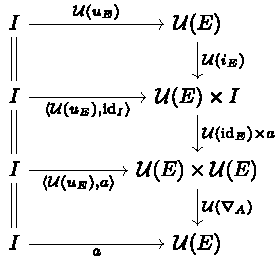
\includegraphics[width=0.95\linewidth,height=0.45\textheight,keepaspectratio]{graphic-15.pdf}\end{center}
    
Observing $\mathcal{D}\left(\operatorname{id}_{I}\rceil a\right)=u_{E}$ (since its domain is $0$), the image under $\mathcal{D}$ of the composite is:\par
    
\begin{center}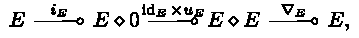
\includegraphics[width=0.95\linewidth,height=0.45\textheight,keepaspectratio]{graphic-16.pdf}\end{center}
    
where (11) gives left- and right-hand morphisms, while Corollary 19 gives the middle morphism. By the left unit law for $i$ and $\nabla$, the composite is the identity, as required. $\hfill\blacktriangleleft$\par
 
% END S3.SS0.SSS0.P0.SPx8.p1
 
% BEGIN S3.SS0.SSS0.P0.SPx8.p2
 
We can use Lemma 22 to strengthen (16): we now consider the differential of a function at any point $a$ and express it with respect to $\overline{\mathsf{d}}$.\par
 
% END S3.SS0.SSS0.P0.SPx8.p2
 
% BEGIN Thmtheorem23
 
\par\medskip\noindent\textbf{Lemma 23.}\par
 
% BEGIN Thmtheorem23.p1
 
For any $a:I\>\vcenter{\hbox{
\includegraphics[height=8.3pt]{inline-36.pdf}}}\>\mathcal{U}(E)$ and $\ell:\oc E\multimap F$, we have:\par
    \[\mathcal{D}\left(a\rceil\ell^{\#}\right)=j_{E};\overline{\mathsf{d}}_{E}\otimes\mathcal{E}^{\prime}(a);\overline{\mathsf{c}}_{E};\ell\]  (18)   
where again $j_{E}:=E\multimap E\otimes 1$ is the inverse of the right unit map.\par
 
% END Thmtheorem23.p1
 
% END Thmtheorem23
 
% END S3.SS0.SSS0.P0.SPx8
 
% BEGIN S3.SS0.SSS0.P0.SPx9
 
\par\medskip\noindent\textbf{Proof.}\par
 
% BEGIN S3.SS0.SSS0.P0.SPx9.p1
 
Consider first the case $\ell=\operatorname{id}_{\oc E}$, so $\ell^{\#}=\eta_{\mathcal{U}(E)}$. By Lemma 22,\par
    \[\mathcal{D}\left(f\rceil\eta_{\mathcal{U}(E)}\right)=\mathcal{D}\left(\mathcal{U}(u_{E})\rceil\mathcal{U}(i_{E});(\operatorname{id}_{\mathcal{U}(E)}\times f);\mathcal{U}(\nabla);\eta_{\mathcal{U}(E)}\right);\]    
By naturality of $\eta$ and monoidality of $\mathcal{E}^{\prime}$, the morphism part of the right-hand side is equal to\par
    \[\left(\oc i_{E};\operatorname{id}_{\oc E}\otimes\mathcal{E}^{\prime}(a);\oc\nabla_{E}\right)^{\#},\]    
whence we can apply (16) to conclude,\par
 
\begin{center}\resizebox{\linewidth}{!}{$\begin{aligned}\displaystyle\mathcal{D}\left(a\rceil\eta_{\mathcal{U}(E)}\right) & \displaystyle=\overline{\mathsf{d}}_{E};\oc i_{E};\operatorname{id}_{\oc E}\otimes\mathcal{E}^{\prime}(a);\overline{\mathsf{c}}_{E}\\\displaystyle=j_{E};\overline{\mathsf{d}}_{E}\otimes\mathcal{E}^{\prime}(a);\overline{\mathsf{c}}_{E}\end{aligned}$}\end{center}
 
by naturality of $j_{E}$ in $E$, observing that $\oc i_{E}=j_{\oc E}$. The general case follows by the argument used to derive (16). $\hfill\blacktriangleleft$\par
 
% END S3.SS0.SSS0.P0.SPx9.p1
 
% BEGIN S3.SS0.SSS0.P0.SPx9.p2
 
We now begin working toward the chain rule, beginning with the context-free case, (6). This turns out to be a consequence of naturality of $\eta$.\par
 
% END S3.SS0.SSS0.P0.SPx9.p2
 
% BEGIN Thmtheorem24
 
\par\medskip\noindent\textbf{Lemma 24.}\par
 
% BEGIN Thmtheorem24.p1
 
For any morphism $a:I\>\vcenter{\hbox{
\includegraphics[height=8.3pt]{inline-37.pdf}}}\>\mathcal{U}(E)$, we have:\par
    \[\mathcal{D}\left(a\rceil\nu_{E}^{\#}\right)=\mathcal{D}\left(a\rceil\eta_{\mathcal{U}(E)}\right);\mathcal{D}\left(a;\eta_{\mathcal{U}(E)}\rceil\eta_{\mathcal{U}(\oc E)}\right)\]  (20)   
% END Thmtheorem24.p1
 
% END Thmtheorem24
 
% END S3.SS0.SSS0.P0.SPx9
 
% BEGIN S3.SS0.SSS0.P0.SPx10
 
\par\medskip\noindent\textbf{Proof.}\par
 
% BEGIN S3.SS0.SSS0.P0.SPx10.p1
 
Recalling that $\nu_{E}=\mathcal{E}^{\prime}\eta_{\mathcal{U}(E)}$, we have a naturality square for $\eta$ that makes the arrows involved equal in $(\mathcal{U}\downarrow\mathscr{C})$, illustrated in the following diagram, to which we apply $\mathcal{D}$:\par
     
\begin{center}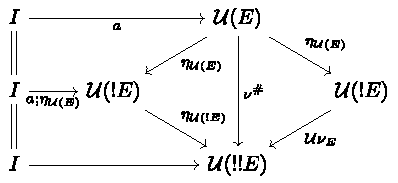
\includegraphics[width=0.95\linewidth,height=0.45\textheight,keepaspectratio]{graphic-17.pdf}\end{center}
      
$\hfill\blacktriangleleft$\par
 
% END S3.SS0.SSS0.P0.SPx10.p1
 
% BEGIN Thmtheorem25
 
\par\medskip\noindent\textbf{Corollary 25.}\par
 
% BEGIN Thmtheorem25.p1
 
The codereliction $\overline{\mathsf{d}}_{A}$ satisfies the chain rule without a context, (6):\par
    \[\overline{\mathsf{d}}_{E};\nu_{E}=j_{E};(\overline{\mathsf{d}}_{E}\otimes\oc u_{E});(\overline{\mathsf{d}}_{\oc E}\otimes\nu_{E});\overline{\mathsf{c}}_{\oc
E}\]  (21)   
% END Thmtheorem25.p1
 
% END Thmtheorem25
 
% END S3.SS0.SSS0.P0.SPx10
 
% BEGIN S3.SS0.SSS0.P0.SPx11
 
\par\medskip\noindent\textbf{Proof.}\par
 
% BEGIN S3.SS0.SSS0.P0.SPx11.p1
 
Let $a=\mathcal{U}(u_{E})$ in (20). We can expand the left-hand side with (16); the first term on the right-hand side is the definition of $\overline{\mathsf{d}}_{E}$ and the second term can be expanded using (19). Observing that $\mathcal{E}^{\prime}(\mathcal{U}(u_{E});\eta_{\mathcal{U}(E)})=\oc u_{A};\nu_{A}$, the resulting identity is:\par
    \[\overline{\mathsf{d}}_{E};\nu_{E}=\overline{\mathsf{d}}_{E};j_{\oc E};\left(\overline{\mathsf{d}}_{\oc E}\otimes(\oc u_{E};\nu_{E})\right);\overline{\mathsf{c}}_{\oc E}.\]    
The right-hand side can be manipulated into the expression in (21) by exploiting naturality of $j$ and rearranging parallel tensored terms. $\hfill\blacktriangleleft$\par
 
% END S3.SS0.SSS0.P0.SPx11.p1
 
% BEGIN S3.SS0.SSS0.P0.SPx11.p2
 
However, to fully interpret $\mathrm{DiLL}$, one also needs to interpret the chain rule within a context (5). This is the translation of a cut rule with a co-dereliction on the context of a promotion in $\mathrm{DiLL}$ with other elements not being cut.\par
 
\begin{center}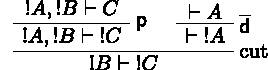
\includegraphics[width=0.95\linewidth,height=0.45\textheight,keepaspectratio]{graphic-18.pdf}\end{center}
 
% END S3.SS0.SSS0.P0.SPx11.p2
 
% BEGIN S3.SS0.SSS0.P0.SPx11.p3
 
Interpreting this rule in the context of Example 14, the proof takes a two-variable function $f:A\times B\>\vcenter{\hbox{
\includegraphics[height=8.3pt]{inline-38.pdf}}}\>C$ (with transpose $f^{\#}:\oc A\otimes\oc B\multimap C$) and promotes it:\par
 
\begin{center}\resizebox{\linewidth}{!}{$\begin{aligned}\displaystyle{\mathsf{p}}(f):\oc A\otimes\oc B & \displaystyle\multimap\oc C;\\\displaystyle\delta_{a}\otimes\delta_{b} & \displaystyle\mapsto\left((g:C\>\vcenter{\hbox{
\includegraphics[height=8.3pt]{inline-39.pdf}}}\>\mathbb{R})\mapsto g(f(a,b))\right).\end{aligned}$}\end{center}
 
Cutting with the codereliction rule means computing, for each vector $v\in A$, the function $\delta_{b}\mapsto\left(g\mapsto D_{(0,b)}(g\circ f)(v,0)\right)$, which expands to, $\delta_{b}\mapsto\left(g\mapsto D_{f(0,b)}g(D_{(0,b)}f)(v,0)\right)$ via the chain rule. Abstracting this reasoning leads us to a “pointed” version of the generalized chain rule.\par
 
% END S3.SS0.SSS0.P0.SPx11.p3
 
% BEGIN Thmtheorem26
 
\par\medskip\noindent\textbf{Proposition 26.}\par
 
% BEGIN Thmtheorem26.p1
 
The codereliction $\overline{\mathsf{d}}_{E}$ satisfies a pointed version of the generalized chain rule (13). Namely, for each $a:I\>\vcenter{\hbox{
\includegraphics[height=8.3pt]{inline-40.pdf}}}\>\mathcal{U}(\oc E)$, we have:\par
 
\begin{center}\resizebox{\linewidth}{!}{$\begin{aligned}\displaystyle\operatorname{id}_{E}\otimes\mathcal{E}^{\prime}(a);\overline{\mathsf{d}}_{E}\otimes\operatorname{id}_{\oc E};\overline{\mathsf{c}}_{E};\nu_{E}=\operatorname{id}_{E}\otimes\mathcal{E}^{\prime}(a);\overline{\mathsf{d}}_{E}\otimes c_{E};\overline{\mathsf{c}}_{E}\otimes\operatorname{id}_{\oc E};\overline{\mathsf{d}}_{\oc E}\otimes\nu_{E};\overline{\mathsf{c}}_{\oc E}.\end{aligned}$}\end{center}
 
% END Thmtheorem26.p1
 
% END Thmtheorem26
 
% END S3.SS0.SSS0.P0.SPx11
 
% BEGIN S3.SS0.SSS0.P0.SPx12
 
\par\medskip\noindent\textbf{Proof.}\par
 
% BEGIN S3.SS0.SSS0.P0.SPx12.p1
 
We deduce the equation from Lemma 24 as follows. By Lemma 23, the left-hand side of (20) expands as:\par
 
\begin{center}\resizebox{\linewidth}{!}{$\begin{aligned}\displaystyle\mathcal{D}\left(a\rceil\nu_{E}^{\#}\right) & \displaystyle=j_{E};\overline{\mathsf{d}}_{E}\otimes\mathcal{E}^{\prime}(a);\overline{\mathsf{c}}_{E};\nu_{E}.\\\displaystyle=j_{E};\operatorname{id}_{E}\otimes\mathcal{E}^{\prime}(a);\overline{\mathsf{d}}_{E}\otimes\operatorname{id}_{\oc E};\overline{\mathsf{c}}_{E};\nu_{E}.\end{aligned}$}\end{center}
 
Meanwhile, the right-hand side expands via two applications of (19) to give:\par
 
\begin{center}\resizebox{\linewidth}{!}{$\begin{aligned}\displaystyle\mathcal{D}\left(a\rceil\nu^{\#}\right) & \displaystyle=j_{E};\overline{\mathsf{d}}_{E}\otimes\mathcal{E}^{\prime}(a);\overline{\mathsf{c}}_{E};j_{\oc E};\overline{\mathsf{d}}_{\oc E}\otimes(\mathcal{E}^{\prime}(a);\nu_{E});\overline{\mathsf{c}}_{\oc E}\\\displaystyle=j_{E};\operatorname{id}_{E}\otimes c_{1};\overline{\mathsf{d}}_{E}\otimes\mathcal{E}^{\prime}(a)\otimes\mathcal{E}^{\prime}(a);\overline{\mathsf{c}}_{E}\otimes\operatorname{id}_{E};\overline{\mathsf{d}}_{\oc E}\otimes\nu_{E};\overline{\mathsf{c}}_{\oc E}\\\displaystyle=j_{E};\operatorname{id}_{E}\otimes\mathcal{E}^{\prime}(a);\overline{\mathsf{d}}_{E}\otimes{\mathsf{c}}_{E};\overline{\mathsf{c}}_{E}\otimes\operatorname{id}_{E};\overline{\mathsf{d}}_{\oc E}\otimes\nu_{E};\overline{\mathsf{c}}_{\oc E}\end{aligned}$}\end{center}
 
Here we pass from the first to the second line by naturality of $j$ and the fact that $j_{E};j_{E\otimes 1}=j_{E};\operatorname{id}_{E}\otimes{\mathsf{c}}_{0}$, and from the second to the third line by naturality of ${\mathsf{c}}$. Since $j_{E}$ is an isomorphism, the desired identity follows. $\hfill\blacktriangleleft$ These developments would be of questionable value if they diverged too far from the established formalism of differential categories, so the following result is important.\par
 
% END S3.SS0.SSS0.P0.SPx12.p1
 

% BEGIN Thmtheorem27
 
\par\medskip\noindent\textbf{Proposition 27.}\par
 
% BEGIN Thmtheorem27.p1
 
A differential category is a functorial model of differentiation (Def.15).\par
 
% END Thmtheorem27.p1
 
% END Thmtheorem27

 
% END S3.SS0.SSS0.P0.SPx12
 

% BEGIN S3.SS0.SSS0.P0.SPx13
 
\par\medskip\noindent\textbf{Proof.}\par
 
% BEGIN S3.SS0.SSS0.P0.SPx13.p1
 
Let $\mathscr{L}$ be a differential category, with notation as in Definition 4. Let us denote by $\mathscr{C}=\mathscr{L}_{\oc}$ the coKleisli category and by $\times$ the product on $\mathscr{L}_{\oc}$ inherited from $\diamond$. Then define a functor $\mathcal{D}:(0\downarrow\mathscr{C})\>\vcenter{\hbox{
\includegraphics[height=8.3pt]{inline-41.pdf}}}\>\mathscr{L}$ by:\par
    \[\mathcal{D}\begin{cases}(a:\oc 0\multimap E)\mapsto E\\
\left(a\rceil g:\oc E\multimap E^{\prime}\right)\mapsto j_{E};(\nu_{0};\oc a)\otimes\overline{\mathsf{d}}_{E};\overline{\mathsf{c}}_{E};g\end{cases}\]    
The effect of $\mathcal{D}$ on morphisms is the exact categorical translation of the effect of $D_{a}g$ in Example 14. To show that $\mathcal{D}$ is functorial, consider:\par
    \[0\xrightarrow{a}E\xrightarrow{g}E^{\prime}\xrightarrow{g^{\prime}}E^{\prime\prime}.\]    
Expanding the definition, we first apply naturality of $j$ and $\nu$, then the argument in the proof of Proposition 26 and naturality of $\overline{\mathsf{c}}$, then naturality of ${\mathsf{c}}$, and finally the chain rule of Definition 4:\par
 
\begin{center}\resizebox{\linewidth}{!}{$\begin{aligned}\displaystyle\mathcal{D}\left(a\rceil g\right) & \displaystyle;\mathcal{D}\left(\nu_{0};\oc a;g\rceil g^{\prime}\right)=j_{E};(\nu_{0};\oc a)\otimes\overline{\mathsf{d}}_{E};\overline{\mathsf{c}}_{E};g;j_{E^{\prime}};(\nu_{0};\oc\nu_{0};\oc\oc a;\oc g)\otimes\overline{\mathsf{d}}_{E^{\prime}};\overline{\mathsf{c}}_{E^{\prime}};g^{\prime}\\\displaystyle=j_{E};\operatorname{id}_{\oc 0}\otimes\left(j_{E};(\nu_{0};\oc a)\otimes\overline{\mathsf{d}}_{E};\overline{\mathsf{c}}_{E}\right);(\nu_{0};\nu_{\oc 0};\oc\oc a;\oc g)\otimes(\overline{\mathsf{d}}_{E};\oc g);\overline{\mathsf{c}}_{\oc E};g^{\prime}\\\displaystyle=j_{E};{\mathsf{c}}_{0}\otimes\operatorname{id}_{E};\operatorname{id}_{\oc 0}\otimes\left((\nu_{0};\oc a)\otimes\overline{\mathsf{d}}_{E};\overline{\mathsf{c}}_{E}\right);(\nu_{0};\oc a;\nu_{E})\otimes\overline{\mathsf{d}}_{E};\overline{\mathsf{c}}_{\oc E};\oc g;g^{\prime}\\\displaystyle=j_{E};(\nu_{0};\oc a)\otimes\operatorname{id}_{E};{\mathsf{c}}_{E}\otimes\overline{\mathsf{d}}_{E};\operatorname{id}_{\oc E}\otimes\overline{\mathsf{c}}_{E};\nu_{E}\otimes\overline{\mathsf{d}}_{E};\overline{\mathsf{c}}_{\oc E};\oc g;g^{\prime}\\\displaystyle=j_{E};(\nu_{0};\oc a)\otimes\operatorname{id}_{E};\operatorname{id}_{\oc E}\otimes\,\overline{\mathsf{d}}_{E};\overline{\mathsf{c}}_{E};\nu_{E};\oc g;g^{\prime}\\\displaystyle=\mathcal{D}\left(a\rceil\nu_{E};\oc g;g^{\prime}\right),\end{aligned}$}\end{center}
 
as required. The fact that $\mathcal{D}\left(a\rceil{\mathsf{d}};\ell\right)=\ell$ follows directly from $\overline{\mathsf{d}};{\mathsf{d}}=\operatorname{id}$, as\par
    \[\mathcal{D}\left(a\rceil{\mathsf{d}};\ell\right)=\oc a\otimes\overline{\mathsf{d}};\overline{\mathsf{c}};{\mathsf{d}};\ell=(\oc a;{\mathsf{d}})\otimes\operatorname{id}_{A};\overline{\mathsf{c}};\ell=\oc u_{A}\otimes\operatorname{id}_{A};\overline{\mathsf{c}};\ell.\ \]    
$\hfill\blacktriangleleft$\par
 
% END S3.SS0.SSS0.P0.SPx13.p1
 
% BEGIN Thmtheorem28
 
\par\medskip\noindent\textbf{$\blacktriangleright$ Remark 28.}\par
 
% BEGIN Thmtheorem28.p1
 
The separation in axiomatic strength between differential categories and our model thus comes down to the separation between the pointed chain rule of Proposition 26 and the generalized version (5). If morphisms of the form $\operatorname{id}_{E}\otimes\mathcal{E}^{\prime}(a)$ are jointly epimorphic (a sort of well-pointedness condition), then the latter follows directly from the former. However, this condition is not satisfied by the category of sets and relations of Example 7 (see [6, section 4]) so this condition seems undesirably strong.\par
 
% END Thmtheorem28.p1
 
% END Thmtheorem28
 
% END S3.SS0.SSS0.P0.SPx13

 
% END S3


% BEGIN S4
 
\par\medskip\noindent\textbf{4 Integration from a functorial point of view}\par
 
% BEGIN S4.p1
 
We now explain how presenting differentiation as a functor on the coslice allows for a new understanding of integration. We begin with a review of integration in Seely categories, based on work by Lemay, Cockett and Ehrhard [7, 11].\par
 
% END S4.p1
 
% BEGIN S4.SS1
 
\par\medskip\noindent\textbf{4.1 Integration and antiderivatives}\par
 
% BEGIN S4.SS1.p1
 
The fundamental theorems of calculus relate differentiation and integration for functions of a single variable. The first (FTC1) states that differentiating the integral of a function returns the original function. For a function $f:\mathbb{R}\mapsto\mathbb{R}$ and $a\in\mathbb{R}$, one has:\par
    \[f(a)=D_{x}\left(x\mapsto\int_{0}^{x}f(t)dt\right)(a).\]    
The second (FTC2) states that integrating a function’s derivative returns the function itself:\par
    \[f=x\mapsto f(a)+\int_{a}^{x}f^{\prime}(t)\,dt.\]    
% END S4.SS1.p1
 
% BEGIN S4.SS1.p2
 
These are valid for real-valued functions only. For higher-order functions, one replaces expressions $f^{\prime}(t)\,dt$ by $D_{a}f(dt)$. This means that integration is an operation on functions with a linear and a non-linear argument:\par
    \[\int_{0}^{a}:(F:\oc A\otimes A\multimap B)\mapsto\left(\left(\int_{0}^{a}F\right):B\right)\]    
% END S4.SS1.p2
 
% BEGIN S4.SS1.p3
 
In Section 3, we considered differentiation at $0$, as encoded by $\overline{\mathsf{d}}$. More generally, we can present differentiation at any point in terms of a so-called deriving transformation.\par
 
% END S4.SS1.p3
 
% BEGIN Thmtheorem29
 
\par\medskip\noindent\textbf{Definition 29.}\par
 
% BEGIN Thmtheorem29.p1
 
In a differential category $\mathscr{L}$, we denote by $\bar{\partial}:\oc\otimes\operatorname{id}\Rightarrow\oc$ the natural transformation:\par
    \[\bar{\partial}_{E}:=\operatorname{id}_{\oc E}\otimes\overline{\mathsf{d}}_{E};\overline{\mathsf{c}}_{E}.\]    
In the context of Example 14, this represents the differential combinator $\delta_{a}\otimes v\mapsto(f\mapsto D_{a}f(v))$. Dually, as introduced by Ehrhard [11], we write ${\partial}:\oc\Rightarrow\oc\otimes\operatorname{id}$ for the natural transformation: ${\partial}_{E}={\mathsf{c}}_{E};\operatorname{id}_{\oc E}\otimes{\mathsf{d}}_{E}$ corresponding to the map $\delta_{v}\mapsto\delta_{v}\otimes v$.\par
 
% END Thmtheorem29.p1
 
% END Thmtheorem29
 
% BEGIN Thmtheorem30
 
\par\medskip\noindent\textbf{Definition 30 ([11]).}\par
 
% BEGIN Thmtheorem30.p1
 
A differential category is said to have antiderivatives if the following morphism is invertible on every object $E$:\par
    \[J_{E}=\operatorname{id}_{\oc E}+({\partial}_{E};\bar{\partial}_{E}):\oc E\multimap\oc E\]    
% END Thmtheorem30.p1
 
% END Thmtheorem30
 
% BEGIN S4.SS1.p4
 
In the distribution model $J_{E}$ would be interpreted as $\delta_{v}\mapsto(f\mapsto f(v)+D_{v}(f)v)$. We refer to [11, section 3.2] for detailed computations using this intuition, which involves integration by parts of the function $x\mapsto\int_{0}^{1}f(tx)dt$.\par
 
% END S4.SS1.p4
 
% BEGIN S4.SS1.p5
 
Lemay and Cockett [7] gave a more general axiomatization of integration independent from differentiation. Integration is represented by a natural transformation $s:\oc A\multimap\oc A\otimes A$. The basic intuition is that post-composing a function $F$ by $s$ results in the integral from zero, $\int_{0}^{\_}F(t,dt)$ where $dt$ stands for any linear argument and not specifically for a measure. Cockett and Lemay then formulate (FTC2) categorically as follows:\par
    \[s;\bar{\partial}+\oc 0=\operatorname{id},\]  (22)   
where $\oc 0={\mathsf{w}};\overline{\mathsf{w}}$. Theorem $(FTC1)$ involves an extra commutativity of variables condition (Poincaré’s lemma), see [11, Prop. 13] and [7, Sec. 5.2]. We leave its study in our context for future work.\par
 
% END S4.SS1.p5
 
% END S4.SS1
 
% BEGIN S4.SS2
 
\par\medskip\noindent\textbf{4.2 Derivatives and Anti-Derivatives in an adjunction}\par
 
% BEGIN S4.SS2.p1
 
Consider a model of Differential Linear Logic, notated as in Definition 4. For the sake of simplicity, we consider $\mathscr{C}$ as the co-Kleisli category over $\mathscr{L}$ for the co-monad $\oc$. We denote $f^{\#}:A\>\vcenter{\hbox{
\includegraphics[height=8.3pt]{inline-42.pdf}}}\>B$ the transpose in $\mathscr{C}$ of the map $f:\oc A\multimap B$ . We still write $\mathcal{U}(\ell)$ for the embedding of a linear map in $\mathscr{C}$, meaning $\mathcal{U}(\ell)=({\mathsf{d}};\ell)^{\#}$.\par
 
% END S4.SS2.p1
 
% BEGIN S4.SS2.p2
 
Note that all statements and proofs, suitably modified, work in the more general context of a linear–non-linear adjunction $\mathcal{E}^{\prime}\dashv\mathcal{U}$, with a functor $\mathcal{D}:(I\downarrow\mathscr{C})\>\vcenter{\hbox{
\includegraphics[height=8.3pt]{inline-43.pdf}}}\>\mathscr{L}$, provided that the generalized chain rule (5) holds: this is used in Proposition 32.\par
 
% END S4.SS2.p2
 
% BEGIN S4.SS2.p3
 
We would like to study a bijection of the following form:\par
    \[\Theta:(I\downarrow\mathscr{C})((A,a),(B,\mathcal{U}(u_{B})))\leftrightarrows\mathscr{L}(\oc A\otimes A,B):\Theta^{-1}\]  (23)   
The core intuition of our development is that $\Theta$ maps a function $f^{\#}:A\rightarrow B$ to its derivative $\overline{\partial};f$. Meanwhile, $\Theta^{-1}$ should map a function $F:\oc A\otimes A\multimap B$ to its integral $s;F:=x\in A\mapsto\int_{a}^{x}F(t,dt)$. Then (FTC1) will translate to $\Theta^{-1};\Theta=\operatorname{id}$. We now develop that statement categorically.\par
 
% END S4.SS2.p3
 
% BEGIN Thmtheorem31
 
\par\medskip\noindent\textbf{Definition 31.}\par
 
% BEGIN Thmtheorem31.p1
 
We define the functor $\mathfrak{D}:(I\downarrow\mathscr{C})\>\vcenter{\hbox{
\includegraphics[height=8.3pt]{inline-44.pdf}}}\>\mathscr{L}$ and the mapping $\Theta$ such that:\par
    \[\mathfrak{D}\colon\left\{\begin{aligned} (a:I\>\vcenter{\hbox{
\includegraphics[height=8.3pt]{inline-45.pdf}}}\>A)&\longmapsto\oc A\otimes A\\
\left(\_\rceil f^{\#}\right)&\longmapsto{\mathsf{c}}_{A}\otimes\operatorname{id}_{A};(\nu;\oc f)\otimes(\bar{\partial}_{A};f)\end{aligned}\right.\kern-1.2pt\]       \[\Theta\colon\left\{\begin{aligned} (I\downarrow\mathscr{C})((A,a),(B,\mathcal{U}(u_{B}))&\longmapsto\mathscr{L}(\mathfrak{D}(A,a),B)\\
\left(\_\rceil f^{\#}\right)&\longmapsto\bar{\partial}_{A};f\end{aligned}\right.\kern-1.2pt\]    
% END Thmtheorem31.p1
 
% END Thmtheorem31
 
% BEGIN S4.SS2.p4
 
With the notation of Section 3 and of Example 6, one has in particular $\mathfrak{D}\left(a\rceil f^{\#}\right)(\delta_{x^{\prime}}\otimes v)=(\delta_{f^{\#}(x^{\prime})})\otimes\mathcal{D}\left(x^{\prime}\rceil f^{\#}\right)$, and $\Theta$ mapping $\left(a\rceil f^{\#}\right)$ to $(\delta_{x^{\prime}}\otimes v)\mapsto\mathcal{D}\left(x^{\prime}\rceil f^{\#}\right)(v)$.\par
 
% END S4.SS2.p4
 
% BEGIN Thmtheorem32
 
\par\medskip\noindent\textbf{Proposition 32.}\par
 
% BEGIN Thmtheorem32.p1
 
$\Theta$ is natural in $A$ and in $B$. If $\Theta$ is moreover an isomorphism, then it defines an adjunction between $\mathfrak{D}$ and the functor $R:B\mapsto(B,u_{B})$ described as a section of $\mathcal{D}$ in the proof of Lemma 21.\par
 
% END Thmtheorem32.p1
 
% END Thmtheorem32
 
% BEGIN S4.SS2.SSS0.P0.SPx1
 
\par\medskip\noindent\textbf{Proof.}\par
 
% BEGIN S4.SS2.SSS0.P0.SPx1.p1
 
Consider morphisms $f^{\#}:(A^{\prime},a^{\prime})\>\vcenter{\hbox{
\includegraphics[height=8.3pt]{inline-46.pdf}}}\>(A,a)$ in $(I\downarrow\mathscr{C})$ and $\ell:B\multimap B^{\prime}\in\mathscr{L}$. To show naturality, one has to prove that $(I\downarrow\mathscr{C})(f^{\#},\mathcal{U}(\ell));\Theta=\Theta;\mathscr{L}(\mathfrak{D}(f)),\ell)$. Consider then $g^{\#}\in(I\downarrow\mathscr{C})((A,a),(B,\mathcal{U}(u_{B}))$. By definition of $\Theta$, $\mathfrak{D}$ and functoriality of $\mathcal{D}$ one has:\par
 
% END S4.SS2.SSS0.P0.SPx1.p1
 
% BEGIN S4.SS2.SSS0.P0.SPx1.p2
 
\begin{center}\resizebox{\linewidth}{!}{$\begin{aligned}\displaystyle\Theta\left(a^{\prime}\rceil f^{\#};g^{\#};\mathcal{U}(\ell)\right) & \displaystyle=\bar{\partial};\nu;\oc\nu;\oc\oc f;\oc g;{\mathsf{d}};\ell=\operatorname{id}\otimes\overline{\mathsf{d}};\nu;\oc\nu;\oc\oc f;\oc g;{\mathsf{d}};\ell\\\displaystyle=\operatorname{id}\otimes\overline{\mathsf{d}};\nu;\oc f;g;\ell\text{ by naturality and comonad laws}\\\displaystyle={\mathsf{c}}_{A^{\prime}}\otimes\overline{\mathsf{d}}_{A^{\prime}};\operatorname{id}\otimes\,\overline{\mathsf{c}}_{A^{\prime}};\nu_{A^{\prime}}\otimes\overline{\mathsf{d}}_{\oc A^{\prime}};\overline{\mathsf{c}}_{\oc A^{\prime}};\oc f;g;\ell\text{ from Equation\leavevmode\nobreak\ (5)}\\\displaystyle(\Theta;\mathscr{L}(\mathfrak{D}(f^{\#})),\ell))(g^{\#}) & \displaystyle=\mathfrak{D}(f^{\#});\Theta\left(a\rceil g^{\#}\right);\ell={\mathsf{c}}_{A^{\prime}}\otimes\operatorname{id}_{A^{\prime}};(\nu;\oc f)\otimes(\bar{\partial}_{A^{\prime}};f);\operatorname{id}\otimes\overline{\mathsf{d}};\overline{\mathsf{c}}_{A};g;\ell\\\displaystyle={\mathsf{c}}_{A^{\prime}}\otimes\operatorname{id}_{A^{\prime}};(\nu;\oc f)\otimes(\operatorname{id}\otimes\overline{\mathsf{d}}_{A^{\prime}};\overline{\mathsf{c}}_{A^{\prime}};f);\operatorname{id}\otimes\overline{\mathsf{d}};\overline{\mathsf{c}}_{A};g;\ell\\\displaystyle={\mathsf{c}}_{A^{\prime}}\otimes\overline{\mathsf{d}}_{A^{\prime}};(\nu;\oc f)\otimes(\overline{\mathsf{c}}_{A^{\prime}};f);\operatorname{id}\otimes\overline{\mathsf{d}};\overline{\mathsf{c}}_{A};g;\ell\\\displaystyle={\mathsf{c}}_{A^{\prime}}\otimes\overline{\mathsf{d}}_{A^{\prime}};\nu\otimes\overline{\mathsf{c}}_{A^{\prime}};\operatorname{id}\otimes\overline{\mathsf{d}};\overline{\mathsf{c}}_{\oc A};\oc f;g;\ell\text{ by naturality of $\overline{\mathsf{d}}$ and $\overline{\mathsf{c}}$}\ \end{aligned}$}\end{center}
 
$\hfill\blacktriangleleft$\par
 
% END S4.SS2.SSS0.P0.SPx1.p2
 
% BEGIN S4.SS2.SSS0.P0.SPx1.p3
 
Note that Equation 23 describe (FTC1) only for functions which are null at some point $a$. Hence, we will need an abelian structure on homsets. Following Proposition 12, $\mathscr{C}(A,gitE)$ has an additive structure ${\boxplus}$ for any $A\in\mathscr{C}$ and $E\in\mathscr{L}$.\par
 
% END S4.SS2.SSS0.P0.SPx1.p3
 
% BEGIN Thmtheorem33
 
\par\medskip\noindent\textbf{Lemma 33.}\par
 
% BEGIN Thmtheorem33.p1
 
For morphisms $\ell,\ell^{\prime}:\oc F\multimap E$ in $\mathscr{L}$, one has $\mathcal{E}^{\prime}(\ell^{\#}\boxplus{\ell^{\prime}}^{\#});{\mathsf{d}}=\ell+\ell^{\prime}$. In particular, when $\mathscr{C}(A,E)$ is an abelian group, transposition across the adjunction preserves subtraction.\par
 
% END Thmtheorem33.p1
 
% END Thmtheorem33
 
% BEGIN S4.SS2.SSS0.P0.SPx1.p4
 
Assuming enrichment in abelian groups, we may now apply $\Theta$ to the translation of $\eta_{A}=\operatorname{id}_{\oc A}^{\#}$ which equals $0$ at $0$, namely $\eta_{A}-{\mathsf{w}}_{A};\overline{\mathsf{w}}_{A};\eta_{A}$. Since $\overline{\mathsf{d}};{\mathsf{w}}=0$, we have:\par
    \[\overline{\partial}=\Theta\left(\mathcal{U}(u_{A})\rceil\eta_{A}-{\mathsf{w}}_{A};\overline{\mathsf{w}}_{A};\eta_{A}\right)\]  (24)   
Define $S_{A}:=\Theta^{-1}(\operatorname{id}_{\oc A\otimes A}):(A,\mathcal{U}(u_{A}))\>\vcenter{\hbox{
\includegraphics[height=8.3pt]{inline-47.pdf}}}\>(\oc A\otimes A,\mathcal{U}(u_{\oc A\otimes A}))$. Intuitively, $S_{A}$ maps a function $F:\oc A\otimes A\multimap A$ to $x\mapsto\int_{0}^{x}F(t,dt)$. Projecting $S_{A}$ in $\mathscr{C}$ one gets $\Pi_{2}(S_{A}):A\>\vcenter{\hbox{
\includegraphics[height=8.3pt]{inline-48.pdf}}}\>\oc A\otimes A$ and as such a morphism of $\mathscr{L}$:\par
    \[s:=\oc A\multimap\oc A\otimes A\]    
% END S4.SS2.SSS0.P0.SPx1.p4
 
% BEGIN Thmtheorem34
 
\par\medskip\noindent\textbf{Proposition 34.}\par
 
% BEGIN Thmtheorem34.p1
 
Consider a functorial model of differentiation, enriched over abelian groups, such that $\mathfrak{D}$ and $R$ form adjunction via (23). Then (FTC2) as formalised in (22) holds.\par
 
% END Thmtheorem34.p1
 
% END Thmtheorem34
 
% END S4.SS2.SSS0.P0.SPx1
 
% BEGIN S4.SS2.SSS0.P0.SPx2
 
\par\medskip\noindent\textbf{Proof.}\par
 
% BEGIN S4.SS2.SSS0.P0.SPx2.p1
 
The proof amounts to a straightforward computation:\par
 
\begin{center}\resizebox{\linewidth}{!}{$\begin{aligned}\displaystyle s;\bar{\partial}+\oc 0 & \displaystyle=\Theta^{-1}(\operatorname{id}_{\oc A\otimes A});\bar{\partial}+{\mathsf{w}}_{A};\overline{\mathsf{w}}_{A}=\Theta^{-1}(\operatorname{id}_{\oc A\otimes A};\bar{\partial})+{\mathsf{w}}_{A};\overline{\mathsf{w}}_{A}\text{ by naturality of $\Theta^{-1}$}\\\displaystyle=\Theta^{-1}(\Theta\left(\mathcal{U}(u_{A})\rceil\eta_{A}-{\mathsf{w}}_{A};bw_{A};\eta_{A}\right))+{\mathsf{w}}_{A};\overline{\mathsf{w}}_{A}\text{ by (24).}\\\displaystyle=\operatorname{id}_{\oc A}-{\mathsf{w}}_{A};\overline{\mathsf{w}}_{A}+{\mathsf{w}}_{A};\overline{\mathsf{w}}_{A}=\operatorname{id}_{\oc A}\text{ by Lemma 33}\ \end{aligned}$}\end{center}
 
$\hfill\blacktriangleleft$\par
 
% END S4.SS2.SSS0.P0.SPx2.p1
 
% END S4.SS2.SSS0.P0.SPx2
 
% END S4.SS2
 
% END S4


% BEGIN S5
 
\par\medskip\noindent\textbf{5 Conclusion}\par
 
% BEGIN S5.p1
 
In this paper, we showed that differentiation as defined in Differential Linear Logic can be described as an extension of the formalism of linear–non-linear adjunction by a functor from a co-slice of the non-linear category to the linear category, $\mathcal{D}:(I\downarrow\mathscr{C})\>\vcenter{\hbox{
\includegraphics[height=8.3pt]{inline-49.pdf}}}\>\mathscr{L}$, and that this recovers differential categories up to a well-pointedness condition. We then extended $\mathcal{D}$ to an adjoint functor in order to describe antiderivatives. We believe that our presentation provides a more accessible axiomatization of differentiation that offers simpler intuitions.\par
 
% END S5.p1
 
% BEGIN S5.p2
 
The following avenues present natural next steps in this research.\par
 
% END S5.p2
 
% BEGIN S5.SS0.SSS0.P0.SPx1
 
\par\medskip\noindent\textbf{Polarity and Differentiation.}\par
 
% BEGIN S5.SS0.SSS0.P0.SPx1.p1
 
Once this work stabilizes, we would like to investigate what polarized models of $\mathrm{DiLL}$ should be, and refine diagram (8) in the case where $\mathscr{L}$ is $\ast$-autonomous, or more generally decomposed into a polarized chirality. One could also use chiralities to relax the coincidence of products and coproducts we relied on in the present paper (constraining us to semi-additive categories) to the mere existence of these structures.\par
 
% END S5.SS0.SSS0.P0.SPx1.p1
 
% END S5.SS0.SSS0.P0.SPx1
 
% BEGIN S5.SS0.SSS0.P0.SPx2
 
\par\medskip\noindent\textbf{Integration.}\par
 
% BEGIN S5.SS0.SSS0.P0.SPx2.p1
 
Section 4 studies integration and (FTC2) only as an inverse to differentiation. A further step in this line of work would be to integrate the formulation of (FTC1) into this presentation. To complement our work on differentiation, we would like to understand how the axioms of integration can be lifted to a functorial presentation on their own to reach a more complete picture of the interactions between integration and differentiation. An interesting question would be whether any adjunction of the form $\mathfrak{D}\dashv R$ results in antiderivatives, in the sense that the natural family of bijections is of the form proposed for $\Theta$ and its inverse.\par
 
% END S5.SS0.SSS0.P0.SPx2.p1
 
% END S5.SS0.SSS0.P0.SPx2
 
% BEGIN S5.SS0.SSS0.P0.SPx3
 
\par\medskip\noindent\textbf{Well-pointedness.}\par
 
% BEGIN S5.SS0.SSS0.P0.SPx3.p1
 
We would like to find an extension of our set-up witnessing the generalized chain rule without recourse to the compromises of Remark 28. An avenue suggested by Zeinab Galal is to extend the domain of definition of $\mathcal{D}$ to a comma category such as $(\mathcal{U}\downarrow\mathscr{C})$ to provide “generalized points” at which to differentiate, possibly abstracting the pairwise functorial differentiation of differentiable programming, $\mathcal{D}(f):\delta_{x}\otimes v\mapsto\delta_{f(x)}\otimes D_{x}f(v)$. This was the origin of the functor $\mathfrak{D}$ used to describe antiderivatives in Section 4.\par
 
% END S5.SS0.SSS0.P0.SPx3.p1
 
% END S5.SS0.SSS0.P0.SPx3
 
% BEGIN S5.SS0.SSS0.P0.SPx4
 
\par\medskip\noindent\textbf{Dependent types.}\par
 
% BEGIN S5.SS0.SSS0.P0.SPx4.p1
 
Finally, this setting gives a dependent flavor to differentiation, and it feels natural to investigate a possible link with dependent types.\par
 
% END S5.SS0.SSS0.P0.SPx4.p1
 
% END S5.SS0.SSS0.P0.SPx4
 
% END S5

\begin{thebibliography}{99}
\bibitem{bib-bib1} 
\par\noindent    R. F. Blute, J. R. B. Cockett, J.-S. P. Lemay, and R. A. G. Seely.  Differential categories revisited.  Applied Categorical Structures, 2020.  doi:10.1007/s10485-019-09572-y.  

\bibitem{bib-bib2} 
\par\noindent    R. F. Blute, J. R. B. Cockett, and R. A. G. Seely.  Differential categories.  Mathematical Structures in Computer Science, 2006.  doi:10.1017/S0960129506005676.  

\bibitem{bib-bib3} 
\par\noindent    R. F. Blute, J. R. B. Cockett, and R. A. G. Seely.  Cartesian differential categories.  Theory and Applications of Categories, 2009.  

\bibitem{bib-bib4} 
\par\noindent    Richard Blute, Thomas Ehrhard, and Christine Tasson.  A convenient differential category.  Cahiers de topologie et géométrie différentielle catégoriques, 53(3):211–232, 2012.  arXiv:1006.3140.  

\bibitem{bib-bib5} 
\par\noindent    A. Brunel, D. Mazza, and M. Pagani.  Backpropagation in the Simply Typed Lambda-calculus with Linear Negation.  POPL, 2020.  doi:10.1145/3371132.  

\bibitem{bib-bib6} 
\par\noindent    Antonio Bucciarelli, Thomas Ehrhard, and Giulio Manzonetto.  Not enough points is enough.  In Computer Science Logic, 2007.  doi:10.1007/978-3-540-74915-8\_24.  

\bibitem{bib-bib7} 
\par\noindent    J. R. B. Cockett and J.-S. Lemay.  Integral categories and calculus categories.  Mathematical Structures in Computer Science, 29:243–308, 2019.  doi:10.1017/S0960129518000014.  

\bibitem{bib-bib8} 
\par\noindent    J. Robin B. Cockett and Geoff S. H. Cruttwell.  Differential Structure, Tangent Structure, and SDG.  Appl. Categorical Struct., 22(2):331–417, 2014.  doi:10.1007/s10485-013-9312-0.  

\bibitem{bib-bib9} 
\par\noindent    J. Robin B. Cockett, Geoff S. H. Cruttwell, Jonathan Gallagher, Jean-Simon Pacaud Lemay, Benjamin MacAdam, Gordon D. Plotkin, and Dorette Pronk.  Reverse derivative categories.  In Maribel Fernández and Anca Muscholl, editors, 28th EACSL Annual Conference on Computer Science Logic, CSL 2020, January 13-16, 2020, Barcelona, Spain, volume 152 of LIPIcs, pages 18:1–18:16. Schloss Dagstuhl – Leibniz-Zentrum für Informatik, 2020.  doi:10.4230/LIPIcs.CSL.2020.18.  

\bibitem{bib-bib10} 
\par\noindent    Y. Dabrowski and M. Kerjean.  Models of Linear Logic based on the Schwartz $\epsilon$ product.  Theory and Applications of Categories, 2020.  doi:10.48550/arXiv.1712.07344.  

\bibitem{bib-bib11} 
\par\noindent    T. Ehrhard.  An introduction to differential linear logic: proof-nets, models and antiderivatives.  Math. Struct. Comput. Sci., 2017.  doi:10.1017/S0960129516000372.  

\bibitem{bib-bib12} 
\par\noindent    T. Ehrhard and L. Regnier.  Differential interaction nets.  Theoretical Computer Science, 364(2), 2006.  doi:10.1016/j.tcs.2006.08.003.  

\bibitem{bib-bib13} 
\par\noindent    Conal Elliott.  The simple essence of automatic differentiation.  In Proceedings of the ACM on Programming Languages (ICFP), 2018.  doi:10.1145/3236765.  

\bibitem{bib-bib14} 
\par\noindent    M. P. Fiore.  Differential structure in models of multiplicative biadditive intuitionistic linear logic.  In TLCA, 2007.  doi:10.1007/978-3-540-73228-0\_13.  

\bibitem{bib-bib15} 
\par\noindent    J.-Y. Girard.  Linear logic.  Theoret. Comput. Sci., 50(1), 1987.  doi:10.1016/0304-3975(87)90045-4.  

\bibitem{bib-bib16} 
\par\noindent    Marie Kerjean.  A logical account for linear partial differential equations.  In Anuj Dawar and Erich Grädel, editors, Proceedings of the 33rd Annual ACM/IEEE Symposium on Logic in Computer Science, LICS 2018, Oxford, UK, July 09-12, 2018, pages 589–598. ACM, 2018.  doi:10.1145/3209108.3209192.  

\bibitem{bib-bib17} 
\par\noindent    Paul-André Mellies.  Categorical semantics of linear logic.  Société Mathématique de France, 2008.  

\bibitem{bib-bib18} 
\par\noindent    L. Schwartz.  Théorie des distributions.  Hermann, Paris, 1966.  

\bibitem{bib-bib19} 
\par\noindent    R. A. G. Seely.  Linear Logic, *-Autonomous Categories and Cofree Coalgebras.  In In Categories in Computer Science and Logic. American Mathematical Society, 1989.  

\end{thebibliography}
\end{document}
